%% 
%% ACS project dissertation template. 
%% 
%% Currently designed for printing two-sided, but if you prefer to 
%% print single-sided just remove ",twoside,openright" from the 
%% \documentclass[] line below. 
%%
%%
%%   SMH, May 2010. 


\documentclass[a4paper,12pt,twoside,openright]{report}


%%
%% EDIT THE BELOW TO CUSTOMIZE
%%

\def\authorname{Francisco A.\ Vargas\xspace}
\def\authorcollege{Girton College\xspace}
\def\authoremail{fav25@cam.ac.uk}
\def\dissertationtitle{Machine Learning Approaches for The Empirical Schrödinger Bridge Problem}
\def\wordcount{200}


%\usepackage[dvips]{epsfig,graphics} 
\usepackage{epsfig,graphicx,verbatim,parskip,tabularx,setspace,xspace}
\usepackage{subfigure}
\usepackage{booktabs}
\usepackage{amsfonts}

\usepackage{natbib}
\usepackage{ marvosym }


\usepackage{tikz}
\usepackage{bayesnet}
\usepackage[linesnumbered, ruled]{algorithm2e}


\usepackage{amsthm}
\usepackage{amsfonts}
\usepackage{amsthm}




%%%%% NEW MATH DEFINITIONS %%%%%

\usepackage{amsmath,amsfonts,bm}

% Mark sections of captions for referring to divisions of figures
\newcommand{\figleft}{{\em (Left)}}
\newcommand{\figcenter}{{\em (Center)}}
\newcommand{\figright}{{\em (Right)}}
\newcommand{\figtop}{{\em (Top)}}
\newcommand{\figbottom}{{\em (Bottom)}}
\newcommand{\captiona}{{\em (a)}}
\newcommand{\captionb}{{\em (b)}}
\newcommand{\captionc}{{\em (c)}}
\newcommand{\captiond}{{\em (d)}}

\newcommand{\sigalg}{{\sigma\text{-algebra}}}

% Highlight a newly defined term
\newcommand{\newterm}[1]{{\bf #1}}


% Figure reference, lower-case.
\def\figref#1{figure~\ref{#1}}
% Figure reference, capital. For start of sentence
\def\Figref#1{Figure~\ref{#1}}
\def\twofigref#1#2{figures \ref{#1} and \ref{#2}}
\def\quadfigref#1#2#3#4{figures \ref{#1}, \ref{#2}, \ref{#3} and \ref{#4}}
% Section reference, lower-case.
\def\secref#1{section~\ref{#1}}
% Section reference, capital.
\def\Secref#1{Section~\ref{#1}}
% Reference to two sections.
\def\twosecrefs#1#2{sections \ref{#1} and \ref{#2}}
% Reference to three sections.
\def\secrefs#1#2#3{sections \ref{#1}, \ref{#2} and \ref{#3}}
% Reference to an equation, lower-case.
\def\eqref#1{equation~\ref{#1}}
% Reference to an equation, upper case
\def\Eqref#1{Equation~\ref{#1}}
% A raw reference to an equation---avoid using if possible
\def\plaineqref#1{\ref{#1}}
% Reference to a chapter, lower-case.
\def\chapref#1{chapter~\ref{#1}}
% Reference to an equation, upper case.
\def\Chapref#1{Chapter~\ref{#1}}
% Reference to a range of chapters
\def\rangechapref#1#2{chapters\ref{#1}--\ref{#2}}
% Reference to an algorithm, lower-case.
\def\algref#1{algorithm~\ref{#1}}
% Reference to an algorithm, upper case.
\def\Algref#1{Algorithm~\ref{#1}}
\def\twoalgref#1#2{algorithms \ref{#1} and \ref{#2}}
\def\Twoalgref#1#2{Algorithms \ref{#1} and \ref{#2}}
% Reference to a part, lower case
\def\partref#1{part~\ref{#1}}
% Reference to a part, upper case
\def\Partref#1{Part~\ref{#1}}
\def\twopartref#1#2{parts \ref{#1} and \ref{#2}}

\def\ceil#1{\lceil #1 \rceil}
\def\floor#1{\lfloor #1 \rfloor}
\def\1{\bm{1}}
\newcommand{\train}{\mathcal{D}}
\newcommand{\valid}{\mathcal{D_{\mathrm{valid}}}}
\newcommand{\test}{\mathcal{D_{\mathrm{test}}}}

\def\eps{{\epsilon}}


% Random variables
\def\reta{{\textnormal{$\eta$}}}
\def\ra{{\textnormal{a}}}
\def\rb{{\textnormal{b}}}
\def\rc{{\textnormal{c}}}
\def\rd{{\textnormal{d}}}
\def\re{{\textnormal{e}}}
\def\rf{{\textnormal{f}}}
\def\rg{{\textnormal{g}}}
\def\rh{{\textnormal{h}}}
\def\ri{{\textnormal{i}}}
\def\rj{{\textnormal{j}}}
\def\rk{{\textnormal{k}}}
\def\rl{{\textnormal{l}}}
% rm is already a command, just don't name any random variables m
\def\rn{{\textnormal{n}}}
\def\ro{{\textnormal{o}}}
\def\rp{{\textnormal{p}}}
\def\rq{{\textnormal{q}}}
\def\rr{{\textnormal{r}}}
\def\rs{{\textnormal{s}}}
\def\rt{{\textnormal{t}}}
\def\ru{{\textnormal{u}}}
\def\rv{{\textnormal{v}}}
\def\rw{{\textnormal{w}}}
\def\rx{{\textnormal{x}}}
\def\ry{{\textnormal{y}}}
\def\rz{{\textnormal{z}}}

% Random vectors
\def\rvepsilon{{\mathbf{\epsilon}}}
\def\rvtheta{{\mathbf{\theta}}}
\def\rva{{\mathbf{a}}}
\def\rvb{{\mathbf{b}}}
\def\rvc{{\mathbf{c}}}
\def\rvd{{\mathbf{d}}}
\def\rve{{\mathbf{e}}}
\def\rvf{{\mathbf{f}}}
\def\rvg{{\mathbf{g}}}
\def\rvh{{\mathbf{h}}}
\def\rvu{{\mathbf{i}}}
\def\rvj{{\mathbf{j}}}
\def\rvk{{\mathbf{k}}}
\def\rvl{{\mathbf{l}}}
\def\rvm{{\mathbf{m}}}
\def\rvn{{\mathbf{n}}}
\def\rvo{{\mathbf{o}}}
\def\rvp{{\mathbf{p}}}
\def\rvq{{\mathbf{q}}}
\def\rvr{{\mathbf{r}}}
\def\rvs{{\mathbf{s}}}
\def\rvt{{\mathbf{t}}}
\def\rvu{{\mathbf{u}}}
\def\rvv{{\mathbf{v}}}
\def\rvw{{\bm{\beta}}}
\def\rvx{{\mathbf{x}}}
\def\rvy{{\mathbf{y}}}
\def\rvz{{\mathbf{z}}}
\def\rvsigma{{\bm{\sigma}}}
\def\rvepsilon{{\bm{\epsilon}}}

% Elements of random vectors
\def\erva{{\textnormal{a}}}
\def\ervb{{\textnormal{b}}}
\def\ervc{{\textnormal{c}}}
\def\ervd{{\textnormal{d}}}
\def\erve{{\textnormal{e}}}
\def\ervf{{\textnormal{f}}}
\def\ervg{{\textnormal{g}}}
\def\ervh{{\textnormal{h}}}
\def\ervi{{\textnormal{i}}}
\def\ervj{{\textnormal{j}}}
\def\ervk{{\textnormal{k}}}
\def\ervl{{\textnormal{l}}}
\def\ervm{{\textnormal{m}}}
\def\ervn{{\textnormal{n}}}
\def\ervo{{\textnormal{o}}}
\def\ervp{{\textnormal{p}}}
\def\ervq{{\textnormal{q}}}
\def\ervr{{\textnormal{r}}}
\def\ervs{{\textnormal{s}}}
\def\ervt{{\textnormal{t}}}
\def\ervu{{\textnormal{u}}}
\def\ervv{{\textnormal{v}}}
\def\ervw{{\textnormal{w}}}
\def\ervx{{\textnormal{x}}}
\def\ervy{{\textnormal{y}}}
\def\ervz{{\textnormal{z}}}

% Random matrices
\def\rmA{{\mathbf{A}}}
\def\rmB{{\mathbf{B}}}
\def\rmC{{\mathbf{C}}}
\def\rmD{{\mathbf{D}}}
\def\rmE{{\mathbf{E}}}
\def\rmF{{\mathbf{F}}}
\def\rmG{{\mathbf{G}}}
\def\rmH{{\mathbf{H}}}
\def\rmI{{\mathbf{I}}}
\def\rmJ{{\mathbf{J}}}
\def\rmK{{\mathbf{K}}}
\def\rmL{{\mathbf{L}}}
\def\rmM{{\mathbf{M}}}
\def\rmN{{\mathbf{N}}}
\def\rmO{{\mathbf{O}}}
\def\rmP{{\mathbf{P}}}
\def\rmQ{{\mathbf{Q}}}
\def\rmR{{\mathbf{R}}}
\def\rmS{{\mathbf{S}}}
\def\rmT{{\mathbf{T}}}
\def\rmU{{\mathbf{U}}}
\def\rmV{{\mathbf{V}}}
\def\rmW{{\mathbf{W}}}
\def\rmX{{\mathbf{X}}}
\def\rmY{{\mathbf{Y}}}
\def\rmZ{{\mathbf{Z}}}

% Elements of random matrices
\def\ermA{{\textnormal{A}}}
\def\ermB{{\textnormal{B}}}
\def\ermC{{\textnormal{C}}}
\def\ermD{{\textnormal{D}}}
\def\ermE{{\textnormal{E}}}
\def\ermF{{\textnormal{F}}}
\def\ermG{{\textnormal{G}}}
\def\ermH{{\textnormal{H}}}
\def\ermI{{\textnormal{I}}}
\def\ermJ{{\textnormal{J}}}
\def\ermK{{\textnormal{K}}}
\def\ermL{{\textnormal{L}}}
\def\ermM{{\textnormal{M}}}
\def\ermN{{\textnormal{N}}}
\def\ermO{{\textnormal{O}}}
\def\ermP{{\textnormal{P}}}
\def\ermQ{{\textnormal{Q}}}
\def\ermR{{\textnormal{R}}}
\def\ermS{{\textnormal{S}}}
\def\ermT{{\textnormal{T}}}
\def\ermU{{\textnormal{U}}}
\def\ermV{{\textnormal{V}}}
\def\ermW{{\textnormal{W}}}
\def\ermX{{\textnormal{X}}}
\def\ermY{{\textnormal{Y}}}
\def\ermZ{{\textnormal{Z}}}

% Vectors
\def\vzero{{\bm{0}}}
\def\vone{{\bm{1}}}
\def\vmu{{\bm{\mu}}}
\def\vtheta{{\bm{\theta}}}
\def\vlambda{{\bm{\lambda}}}
\def\va{{\bm{a}}}
\def\vb{{\bm{b}}}
\def\vc{{\bm{c}}}
\def\vd{{\bm{d}}}
\def\ve{{\bm{e}}}
\def\vf{{\bm{f}}}
\def\vg{{\bm{g}}}
\def\vh{{\bm{h}}}
\def\vi{{\bm{i}}}
\def\vj{{\bm{j}}}
\def\vk{{\bm{k}}}
\def\vl{{\bm{l}}}
\def\vm{{\bm{m}}}
\def\vn{{\bm{n}}}
\def\vo{{\bm{o}}}
\def\vp{{\bm{p}}}
\def\vq{{\bm{q}}}
\def\vr{{\bm{r}}}
\def\vs{{\bm{s}}}
\def\vt{{\bm{t}}}
\def\vu{{\bm{u}}}
\def\vv{{\bm{v}}}
\def\vw{{\bm{w}}}
\def\vx{{\bm{x}}}
\def\vy{{\bm{y}}}
\def\vz{{\bm{z}}}

% Elements of vectors
\def\evalpha{{\alpha}}
\def\evbeta{{\beta}}
\def\evepsilon{{\epsilon}}
\def\evlambda{{\lambda}}
\def\evomega{{\omega}}
\def\evmu{{\mu}}
\def\evpsi{{\psi}}
\def\evsigma{{\sigma}}
\def\evtheta{{\theta}}
\def\eva{{a}}
\def\evb{{b}}
\def\evc{{c}}
\def\evd{{d}}
\def\eve{{e}}
\def\evf{{f}}
\def\evg{{g}}
\def\evh{{h}}
\def\evi{{i}}
\def\evj{{j}}
\def\evk{{k}}
\def\evl{{l}}
\def\evm{{m}}
\def\evn{{n}}
\def\evo{{o}}
\def\evp{{p}}
\def\evq{{q}}
\def\evr{{r}}
\def\evs{{s}}
\def\evt{{t}}
\def\evu{{u}}
\def\evv{{v}}
\def\evw{{w}}
\def\evx{{x}}
\def\evy{{y}}
\def\evz{{z}}

% Matrix
\def\mA{{\bm{A}}}
\def\mB{{\bm{B}}}
\def\mC{{\bm{C}}}
\def\mD{{\bm{D}}}
\def\mE{{\bm{E}}}
\def\mF{{\bm{F}}}
\def\mG{{\bm{G}}}
\def\mH{{\bm{H}}}
\def\mI{{\bm{I}}}
\def\mJ{{\bm{J}}}
\def\mK{{\bm{K}}}
\def\mL{{\bm{L}}}
\def\mM{{\bm{M}}}
\def\mN{{\bm{N}}}
\def\mO{{\bm{O}}}
\def\mP{{\bm{P}}}
\def\mQ{{\bm{Q}}}
\def\mR{{\bm{R}}}
\def\mS{{\bm{S}}}
\def\mT{{\bm{T}}}
\def\mU{{\bm{U}}}
\def\mV{{\bm{V}}}
\def\mW{{\bm{W}}}
\def\mX{{\bm{X}}}
\def\mY{{\bm{Y}}}
\def\mZ{{\bm{Z}}}
\def\mBeta{{\bm{\beta}}}
\def\mPhi{{\bm{\Phi}}}
\def\mLambda{{\bm{\Lambda}}}
\def\mSigma{{\bm{\Sigma}}}

% Tensor
\DeclareMathAlphabet{\mathsfit}{\encodingdefault}{\sfdefault}{m}{sl}
\SetMathAlphabet{\mathsfit}{bold}{\encodingdefault}{\sfdefault}{bx}{n}
\newcommand{\tens}[1]{\bm{\mathsfit{#1}}}
\def\tA{{\tens{A}}}
\def\tB{{\tens{B}}}
\def\tC{{\tens{C}}}
\def\tD{{\tens{D}}}
\def\tE{{\tens{E}}}
\def\tF{{\tens{F}}}
\def\tG{{\tens{G}}}
\def\tH{{\tens{H}}}
\def\tI{{\tens{I}}}
\def\tJ{{\tens{J}}}
\def\tK{{\tens{K}}}
\def\tL{{\tens{L}}}
\def\tM{{\tens{M}}}
\def\tN{{\tens{N}}}
\def\tO{{\tens{O}}}
\def\tP{{\tens{P}}}
\def\tQ{{\tens{Q}}}
\def\tR{{\tens{R}}}
\def\tS{{\tens{S}}}
\def\tT{{\tens{T}}}
\def\tU{{\tens{U}}}
\def\tV{{\tens{V}}}
\def\tW{{\tens{W}}}
\def\tX{{\tens{X}}}
\def\tY{{\tens{Y}}}
\def\tYQ{{\tens{{\:}_q\!Y}}}
\def\tZ{{\tens{Z}}}


% Graph
\def\gA{{\mathcal{A}}}
\def\gB{{\mathcal{B}}}
\def\gC{{\mathcal{C}}}
\def\gD{{\mathcal{D}}}
\def\gE{{\mathcal{E}}}
\def\gF{{\mathcal{F}}}
\def\gG{{\mathcal{G}}}
\def\gH{{\mathcal{H}}}
\def\gI{{\mathcal{I}}}
\def\gJ{{\mathcal{J}}}
\def\gK{{\mathcal{K}}}
\def\gL{{\mathcal{L}}}
\def\gM{{\mathcal{M}}}
\def\gN{{\mathcal{N}}}
\def\gO{{\mathcal{O}}}
\def\gP{{\mathcal{P}}}
\def\gQ{{\mathcal{Q}}}
\def\gR{{\mathcal{R}}}
\def\gS{{\mathcal{S}}}
\def\gT{{\mathcal{T}}}
\def\gU{{\mathcal{U}}}
\def\gV{{\mathcal{V}}}
\def\gW{{\mathcal{W}}}
\def\gX{{\mathcal{X}}}
\def\gY{{\mathcal{Y}}}
\def\gZ{{\mathcal{Z}}}

% Sets
\def\sA{{\mathbb{A}}}
\def\sB{{\mathbb{B}}}
\def\sC{{\mathbb{C}}}
\def\sD{{\mathbb{D}}}
% Don't use a set called E, because this would be the same as our symbol
% for expectation.
\def\sF{{\mathbb{F}}}
\def\sG{{\mathbb{G}}}
\def\sH{{\mathbb{H}}}
\def\sI{{\mathbb{I}}}
\def\sJ{{\mathbb{J}}}
\def\sK{{\mathbb{K}}}
\def\sL{{\mathbb{L}}}
\def\sM{{\mathbb{M}}}
\def\sN{{\mathbb{N}}}
\def\sO{{\mathbb{O}}}
\def\sP{{\mathbb{P}}}
\def\sQ{{\mathbb{Q}}}
\def\sR{{\mathbb{R}}}
\def\sS{{\mathbb{S}}}
\def\sT{{\mathbb{T}}}
\def\sU{{\mathbb{U}}}
\def\sV{{\mathbb{V}}}
\def\sW{{\mathbb{W}}}
\def\sX{{\mathbb{X}}}
\def\sY{{\mathbb{Y}}}
\def\sZ{{\mathbb{Z}}}

% Entries of a matrix
\def\emLambda{{\Lambda}}
\def\emA{{A}}
\def\emB{{B}}
\def\emC{{C}}
\def\emD{{D}}
\def\emE{{E}}
\def\emF{{F}}
\def\emG{{G}}
\def\emH{{H}}
\def\emI{{I}}
\def\emJ{{J}}
\def\emK{{K}}
\def\emL{{L}}
\def\emM{{M}}
\def\emN{{N}}
\def\emO{{O}}
\def\emP{{P}}
\def\emQ{{Q}}
\def\emR{{R}}
\def\emS{{S}}
\def\emT{{T}}
\def\emU{{U}}
\def\emV{{V}}
\def\emW{{W}}
\def\emX{{X}}
\def\emY{{Y}}
\def\emZ{{Z}}
\def\emSigma{{\Sigma}}

% entries of a tensor
% Same font as tensor, without \bm wrapper
\newcommand{\etens}[1]{\mathsfit{#1}}
\def\etLambda{{\etens{\Lambda}}}
\def\etA{{\etens{A}}}
\def\etB{{\etens{B}}}
\def\etC{{\etens{C}}}
\def\etD{{\etens{D}}}
\def\etE{{\etens{E}}}
\def\etF{{\etens{F}}}
\def\etG{{\etens{G}}}
\def\etH{{\etens{H}}}
\def\etI{{\etens{I}}}
\def\etJ{{\etens{J}}}
\def\etK{{\etens{K}}}
\def\etL{{\etens{L}}}
\def\etM{{\etens{M}}}
\def\etN{{\etens{N}}}
\def\etO{{\etens{O}}}
\def\etP{{\etens{P}}}
\def\etQ{{\etens{Q}}}
\def\etR{{\etens{R}}}
\def\etS{{\etens{S}}}
\def\etT{{\etens{T}}}
\def\etU{{\etens{U}}}
\def\etV{{\etens{V}}}
\def\etW{{\etens{W}}}
\def\etX{{\etens{X}}}
\def\etY{{\etens{Y}}}
\def\etZ{{\etens{Z}}}


\def\uni{{\text{Uniform}}}
\def\gam{{\text{Gamma}}}
\def\erf{{\text{erf}}}
\def\sigms{{\text{sigmoid}}}
% \def\softplus{{\text{softplus}}}
\def\logit{{\text{logit}}}
\def\bdist{{\text{Beta}}}
\def\dir{{\text{Dir}}}
\def\cat{{\text{Cat}}}
\def\bern{{\text{Bernoulli}}}
\def\NN{{\text{NN}}}
\def\yset{{\{y_i\}}}
\def\xset{{\{\vx_i\}}}
\def\tset{{\{\theta_i\}}}
\def\uchi{{\Phi_{\vx_i, \vlambda}^{-1}(u)}}
\def\uchic{{\Phi_{\vx_i, \vlambda,c}^{-1}(u)}}
\def\uchj{{\Phi_{\vx_j, \vlambda}^{-1}(u)}}
\def\uchkij{{\Phi_{\vx_i, \vlambda}^{-1}(\Phi_{\vx_j, \vlambda}(v))}}
\def\uchkijt{{\Phi_{\vx_i, \vlambda}^{-1}(\Phi_{\vx_j, \vlambda}(\theta_j))}}
\def\uch{{\Phi_{\vx^*, \vlambda}^{-1}(u)}}
\def\uchis{{\Phi_{\vx_i, \vlambda}^{-1}(u_{(s)})}}
\def\uchih{{\Phi_{\vx_i, \hat{\vlambda}}^{-1}(u)}}
\def\uchh{{\Phi_{\vx^*, \hat{\vlambda} }^{-1}(u)}}

% \def\logsumexp{{\text{logsumexp}}}

% The true underlying data generating distribution
\newcommand{\pdata}{p_{\rm{data}}}
% The empirical distribution defined by the training set
\newcommand{\ptrain}{\hat{p}_{\rm{data}}}
\newcommand{\Ptrain}{\hat{P}_{\rm{data}}}
% The model distribution
\newcommand{\pmodel}{p_{\rm{model}}}
\newcommand{\Pmodel}{P_{\rm{model}}}
\newcommand{\ptildemodel}{\tilde{p}_{\rm{model}}}
% Stochastic autoencoder distributions
\newcommand{\pencode}{p_{\rm{encoder}}}
\newcommand{\pdecode}{p_{\rm{decoder}}}
\newcommand{\precons}{p_{\rm{reconstruct}}}

\newcommand{\laplace}{\mathrm{Laplace}} % Laplace distribution

\newcommand{\E}{\mathbb{E}}
\newcommand{\W}{\mathbb{W}}
\newcommand{\Ls}{\mathcal{L}}
\newcommand{\R}{\mathbb{R}}
\newcommand{\emp}{\tilde{p}}
\newcommand{\lr}{\alpha}
\newcommand{\reg}{\lambda}
\newcommand{\rect}{\mathrm{rectifier}}
\newcommand{\softmax}{\mathrm{softmax}}
\newcommand{\sigmoid}{\sigma}
\newcommand{\softplus}{{\text{softplus}}}

\def\calP{{\mathcal{P}}}
\def\calD{{\mathcal{D}}}
\def\calF{{\mathcal{F}}}
\def\calQ{{\mathcal{Q}}}
\def\calB{{\mathcal{B}}}
\def\calN{{\mathcal{N}}}
\def\calL{{\mathcal{L}}}
\def\callambda{{\mathcal{\lambda}}}
\def\calW{{\mathcal{W}}}
\def\calT{{\mathcal{T}}}

\def\calH{{\mathcal{H}}}


\let\log\relax
\DeclareMathOperator{\log}{ln}

\def\P{{\mathbb{P}}}
\def\F{{\mathbb{F}}}
\def\Q{{\mathbb{Q}}}
\def\B{{\mathbb{B}}}
\def\I{{\mathbb{I}_d}}
\def\ind{{\bm{1}}}
\def\R{{\mathbb{R}}}
\def\X{{\mathbb{X}}}


\def\hphi{{\hat{\phi}}}


% \def\KL{{D_{\text{KL}}}}

\newcommand{\indep}{\raisebox{0.05em}{\rotatebox[origin=c]{90}{$\models$}}}


\newcommand\independent{\protect\mathpalette{\protect\independenT}{\perp}}
\def\independenT#1#2{\mathrel{\rlap{$#1#2$}\mkern2mu{#1#2}}}

\def\probspace{{(\Omega, \mathcal{F}, \mathbb{P})}}
\def\filtprobspace{{(\Omega, \mathcal{F}, \mathfrak{F}, \mathbb{P})}}

\newcommand{\KL}{D_{\mathrm{KL}}}
\newcommand{\Var}{\mathrm{Var}}
\newcommand{\standarderror}{\mathrm{SE}}
\newcommand{\Cov}{\mathrm{Cov}}
% Wolfram Mathworld says $L^2$ is for function spaces and $\ell^2$ is for vectors
% But then they seem to use $L^2$ for vectors throughout the site, and so does
% wikipedia.
\newcommand{\normlzero}{L^0}
\newcommand{\normlone}{L^1}
\newcommand{\normltwo}{L^2}
\newcommand{\normlp}{L^p}
\newcommand{\normmax}{L^\infty}

\def\vec{{\text{vec}}}

\newcommand{\parents}{Pa} % See usage in notation.tex. Chosen to match Daphne's book.

\DeclareMathOperator*{\argmax}{arg\,max}
\DeclareMathOperator*{\argmin}{arg\,min}
\DeclareMathOperator*{\arginf}{arg\,inf}
\DeclareMathOperator*{\argsup}{arg\,sup}
\DeclareMathOperator*{\logsumexp}{logsumexp}

\def\kk{{\text{k}}}

\DeclareMathOperator{\sign}{sign}
\DeclareMathOperator{\Tr}{Tr}
\let\ab\allowbreak


\newtheorem{theorem}{Theorem}
\newtheorem{corollary}{Corollary}[theorem]
\newtheorem{lemma}[theorem]{Lemma}
\newtheorem{proposition}[theorem]{Proposition}
\newtheorem{observation}[theorem]{Observation}
\theoremstyle{definition}
\newtheorem{definition}{Definition}[section]

\makeatletter
\def\mathcolor#1#{\@mathcolor{#1}}
\def\@mathcolor#1#2#3{%
  \protect\leavevmode
  \begingroup
    \color#1{#2}#3%
  \endgroup
}
\makeatother


%% START OF DOCUMENT
\begin{document}


%% FRONTMATTER (TITLE PAGE, DECLARATION, ABSTRACT, ETC) 
\pagestyle{empty}
\singlespacing
% title page information
\begin{titlepage} 

\begin{center}
\noindent
\huge
\dissertationtitle \\
\vspace*{\stretch{1}}
\end{center}

\begin{center}
\noindent
\huge
\authorname \\
\Large
\authorcollege      \\[24pt]
%\begin{figure}

\includegraphics{CUni3.pdf}
%\end{figure}
\end{center}

\vspace{24pt} 

\begin{center}
\noindent
\large
{\it A dissertation submitted to the University of Cambridge \\ 
in partial fulfilment of the requirements for the degree of \\ 
Master of Philosophy in Advanced Computer Science} 
\vspace*{\stretch{1}}
\end{center}

\begin{center}
\noindent
University of Cambridge \\
Computer Laboratory     \\
William Gates Building  \\
15 JJ Thomson Avenue    \\
Cambridge CB3 0FD       \\
{\sc United Kingdom}    \\
\end{center}

\begin{center}
\noindent
Email: \authoremail \\
\end{center}

\begin{center}
\noindent
\today
\end{center}

\end{titlepage} 

\newpage
\vspace*{\fill}

\onehalfspacing
\newpage
%TC:ignore
{\Huge \bf Declaration}

\vspace{24pt} 

I \authorname of \authorcollege, being a candidate for the M.Phil in
Advanced Computer Science, hereby declare that this report and the
work described in it are my own work, unaided except as may be
specified below, and that the report does not contain material that
has already been used to any substantial extent for a comparable
purpose.

\vspace{24pt}
Total word count: \wordcount

\vspace{60pt}
\textbf{Signed}: 

\vspace{12pt}
\textbf{Date}:


\vfill

This dissertation is copyright \copyright 2020 \authorname. 
\\
All trademarks used in this dissertation are hereby acknowledged.



\newpage
\vspace*{\fill}
%TC:endignore
\singlespacing
\newpage
{\Huge \bf Abstract}
\vspace{24pt} 


The Schrödinger bridge problem is concerned with finding the most likely stochastic evolution between two probability distributions given a prior/reference stochastic evolution. This problem was posed by Schrödinger in \cite{schrodinger1931uber,schrodinger1932theorie} and solved to a large extent. Problems of this kind, whilst not popular in the machine learning community, have direct applications such as Domain Adaptation, Hypothesis Testing, Semantic Similarity, and others.

Thus, the focus of this thesis is to carry out a preliminary study on computational approaches for estimating the Schrödinger bridge between two distributions, when these distributions are available (or can be available) through samples, as most problems in Machine Learning are.

Due to the mathematical nature of the problem, this manuscript is partly concerned with restating and re-deriving many theorems and results that are either overlooked within the mathematical community or hidden in type-written textbooks behind paywalls. Part of the aim of this sub-goal is to make the mathematical toolery behind these approaches more accessible to a broader scientific and engineering audience.

\newpage
\vspace*{\fill}


\pagenumbering{roman}
\setcounter{page}{0}
\pagestyle{plain}
\tableofcontents
\listoffigures
\listoftables

\onehalfspacing

%% START OF MAIN TEXT 

 \chapter{Introduction}
 \pagenumbering{arabic} 
 
 The motion of small particles in a fluid and the value of financial instruments as a function of time have an interesting intersection. These two processes have a large number of underlying factors (i.e. physical forces) that impact their trajectories and constantly change as a function of time. This dramatic and constant stream of varying forces cause the trajectory of these systems to seem random and make it unfeasible to model with classical physics. 
 
 What we today call Brownian motion is a random process and one of the simplest physical models that is used to describe the motion of small particles in a fluid. Some of the earliest mathematical formulations of this process date back to \cite{einstein1905motion}, where the diffusion-based formulation of Brownian motion was used to describe the motion of pollen particles in a fluid.
 
 As one then may naturally and accurately conjecture, many day-to-day processes have an element of Brownian motion within them, and thus Brownian motion has become a substantial mathematical tool when describing the motion of volatile temporal processes.
 
 A class of Brownian-motion-driven processes that are of particular interest to many areas of applied science are the drift-augmented Brownian motions. In simple terms, this family of processes can be split into two components: one being a Brownian-motion-driven term and the other being a drift which provides a directional drive to the system, much like a driving force.  A particular example process that is popular in the Machine Learning and Computational Neuroscience communities is the Ornstein–Uhlenbeck (OU) process. The OU-process is used to model particles undergoing Brownian motion that are subject to friction, here the drift term represents the friction. Another interesting remark is that the discrete-time analogue of the OU-process is the auto-regressive process of order $1$ -- $\text{AR}(1)$, which has multiple uses in time-series analysis and signal processing. Whilst in practice these processes are discretised, their continuous time formulation remain useful objects for the study of their theoretical properties.
 
 This project is concerned with a specific event regarding Brownian-motion-driven processes proposed by Schrödinger in \citep{schrodinger1931uber, schrodinger1932theorie} . The event proposes a group of particles undergoing Brownian motion in $\R^d$, where we observe their position distributions $\pi_0(x)$ at time $0$, and then $\pi_1(y)$ at time $1$. Then, consider the case where $\pi_1(y)$ differs significantly from the predicted distribution by Brownian motion, that is
 \begin{align*}
     \pi_1(y) \neq \int p(x, 0, y , 1) \pi_1(x) dx,
 \end{align*}
 where $p(x, 0, y , 1) = p(y_1| x_0)$ represents the transition density under the Brownian motion, that is, the probability of transitioning from $x$ at time $0$ to $y$ at time $1$. We can model this event as the particles at time $0$ were transported to time $1$ in an unlikely manner (a rare event). Out of the many unlikely ways in which this event could have happened, the Schrödinger bridge answers the question of which one is the most likely. We will see down the line that this question boils down to finding a drift-augmented Brownian motion that satisfies the observed distributions and is as close to Brownian motion as possible in a KL-divergence sense.
 
 Rephrasing this in a more machine learning setting, the Schrödinger bridge is concerned with finding the most likely stochastic process that evolves a distribution $\pi_0(x)$ to another distribution $\pi_1(y)$, and is in line with a pre-specified Brownian motion prior.
 
 From an application viewpoint, the Schrödinger bridge provides us with a well-grounded mechanism for mapping between two distributions, and when those distributions are only available through samples, we effectively have a classical, unsupervised domain-adaptation problem, as illustrated in Figure \ref{fig:intuitive_bridge}. Furthermore, the Schrödinger bridge also provides us with the probability of this stochastic evolution, thus allowing us to compare two data sets/distributions which can be useful for hypothesis testing and semantic similarly.
 
 In this project will be exploring machine learning based approaches to estimate the Schrödinger bridge between two distributions that are available through samples.
\begin{figure}
    \centering
    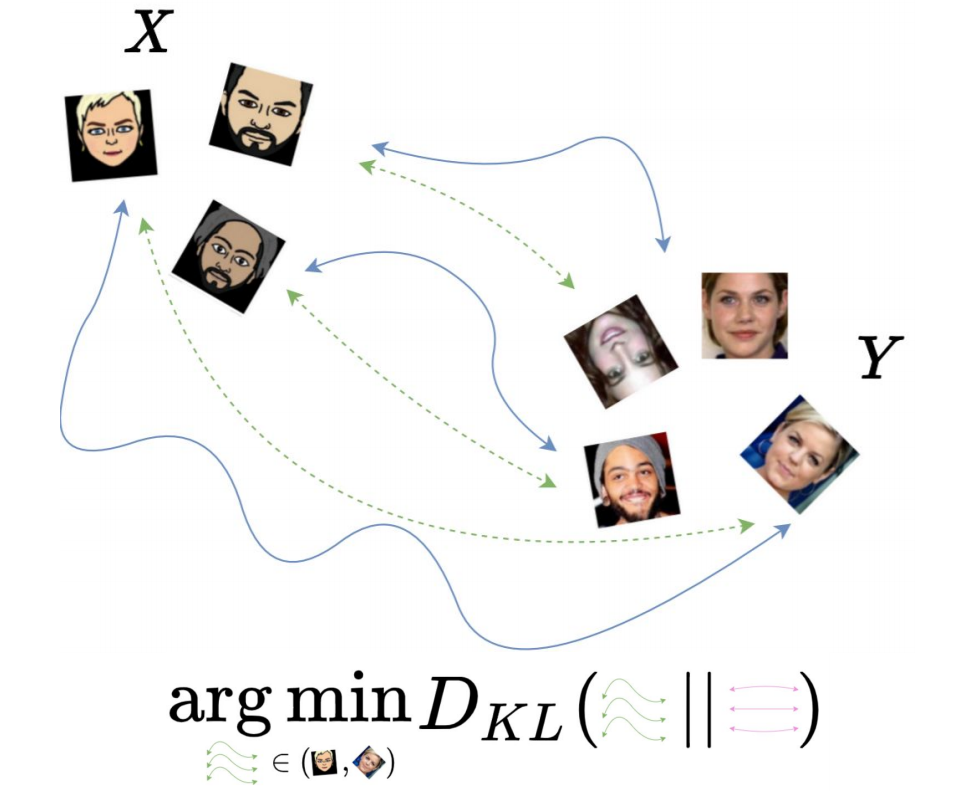
\includegraphics[scale=0.7]{images/charicaturistic_bridge.PNG}
    \caption{Intuitive Illustration of the Schrödinger Bridge}
    \label{fig:intuitive_bridge}
\end{figure}

 
\chapter{Mathematical Preliminaries}

\setcounter{page}{1}

The goal of this chapter is to introduce mathematical notation, concepts and lemmas that we will make use of throughout this study. Whilst many of these lemmas seem to be omitted as steps or taken for granted in the stochastic process literature, we found that some of them were not directly accessible when searched for and not taught in graduate-level measure and probability theory courses. Therefore, it will be useful for the community to restate and re-derive some of these results, in order to make the theory behind Schrödinger Bridges more accessible to the computational sciences.
\section{Probability Space Formalism}

For many of the technical derivations in the methodology we will study, a basic notion of measure and integration is required, thus we will refresh concepts such as $\sigalg$, probability measures,  measurable functions and the Lebesgue–Stieltjes integral, without going into unnecessary technical detail.

\begin{definition} \label{def:prob_space}
A probability space is defined as a 3-element tuple $\probspace$, where:
\begin{itemize}
    \item $\Omega$ is the sample space, i.e. the set of possible outcomes. For example, for a coin toss $\Omega=\{\text{Head}, \text{Tails}\}$. 
    \item The $\sigalg$ $\mathcal{F} \subseteq 2^{\Omega}$ which represents the set of events we may want to consider. Continuing the coin toss example, we may have $\Omega=\{\emptyset, \text{Head}, \text{Tails},\{\text{Head}, \text{Tails}\}\}$.
    \item A probability measure $\P:\calF \rightarrow [0,1]$, which is a function which assigns a number in $[0,1]$ to any event (set) in the $\sigalg$ $\calF$. The function $\P$ has the following requirements:
    \begin{itemize}
        \item $\sigma$-additive (also called countable additive), which means that if  $\bigcup_{i=0}^\infty  A_i\in \calF$ and $A_j \cap A_j = \emptyset, \; i \neq j$then $\P\left(\bigcup_{i=0}^\infty A_i\right) =\sum_{i=0}^\infty \P(A_i) $.
        \item $\P(\Omega)=1$, which we can read as the sample space summing up to (integrating) to 1.  Without this condition $\P$ would be a regular measure ($\sigma$-additive).
    \end{itemize}
\end{itemize}
\end{definition}
One thing to note from the above definition is that we want to be able to measure (assign a value/probability to a set) to each set in $\calF$, and this is not always possible. In other words, one can construct sets that cannot be measured (or can only be measured by the trivial measure $\callambda(A) = 0$, which is not a probability measure). Thus, we require $\calF$ to only contain measurable sets and this is what a $\sigalg$ guarantees:
\begin{definition}\label{def:sigma_algebra}
A $\sigalg$ $\calF \subseteq 2^{\Omega}$ is a collection of sets satisfying the property:
\begin{itemize}
    \item $\calF$ contains $\Omega$: $\Omega \in \calF$.
    \item $\calF$ is closed under complements: if $A\in\calF$, then $\Omega \setminus A \in \calF$.
    \item $\calF$ is closed under countable union:  if $A_i \in \calF$ then $\bigcup_i A_i \in \calF$.
\end{itemize}
\end{definition}

Note we use the notation $\calB(\R^d)$ for the Borel Sigma Algebra of of $\R^d$ which we can think of this as the canonical sigma algebra for $\R^d$, it is the most compact representation of all measurable sets in $\R^d$. This notation can also be extended for subsets of $\R^d$ and in more general any topological space,.

\begin{definition}\label{def:random_variable}
For a probability space $\probspace$, real-valued random variable (vector) $\rvx(\omega)$ is a function $\rvx :\Omega \rightarrow \R^d$, with the requirement that $\rvx(\omega)$ is a measurable function, meaning that the pre-image of $\rvx(\omega)$  lies within the $\sigalg$ $\calF$:
\begin{align*}
    \rvx^{-1}(B)= \{\omega : \rvx(\omega) \in B \} \in \calF .
\end{align*}
\end{definition}
Effectively, the above formalism of the random variable allows us to assign a numerical representation to outcomes in $\Omega$. The clear advantage is that now we can ask questions, such as what the probability that $\rvx$ is contained within a set $B \subseteq \R^d$ is:
\begin{align*}
     \text{P}(\rvx(\omega) \in B) = \P( \{\omega : \rvx(\omega) \in B \} ),
\end{align*}
 and if we consider the more familiar 1D example, we recover the cumulative distribution function (CDF):
 \begin{align*}
     \text{P}(\rx(\omega) \leq r) = \P( \{\omega : \rx(\omega) \leq r \} ).
 \end{align*}
 The random-variable formalism provides us with a more clear connection between the probability measure $\P$ and the more familiar CDF. For simplicity in some cases, we may drop the argument $\omega$ from the random variable notation (i.e $\rvx \sim \calN(\bm{0}, \mathbb{I})$). 

\subsection{Lebesgue–Stieltjes Integral}
Here we will attempt a pragmatic introduction to the Lebesgue–Stieltjes integral, in the context of a probability space. For a more technical introduction, we point the reader to advanced probability theory or measure and integration courses.
\begin{definition}\label{def:lebesgue}
For a probability measure space $\probspace$ and a measurable function $f: \Omega \rightarrow \R $, and $A \in \calF$ the Lebesgue–Stieltjes integral
\begin{align}
    \int_{A} f(\vx) d\P(\vx)
\end{align}
is the Lebesgue integral with respect to the probability measure $\P$.
\end{definition}
Whilst we have not yet introduced a precise definition for the Lebesgue integral, we will now illustrate some of its properties that give us a grasp of this seemingly new notation:
Expectations in our probability space can be written as
\begin{align}
     \E_{\P}[f(\rvx)] = \int_{\Omega} f(\vx) d\P(\vx).
\end{align}
Let $\ind(\rvx \in A)$ be the indicator function for set $A$, then
\begin{align}
    \E_{\P}[\ind(\rvx \in A)] = \int_{\Omega} \ind(\rvx \in A) d\P(\vx) = \int_{A} d\P(\vx) = \P(A).
\end{align}
The above result is a useful example, since it shows us how the distribution (probability measure) is defined in terms of the integral. This is effectively  the definition of a cumulative density function.
When our distribution $\P$ admits a probability density function $p(\vx)$, we have the following:
\begin{align}
    \int_{\Omega} f(\vx) d\P(\vx) = \int_{\Omega} f(\vx)p(\vx) d\callambda(\vx),
\end{align}
where $\callambda$ is the Lesbesgue measure and we can just think of it as the characteristic measure for $\R^d$. For many purposes we can just interpret $\int_{\Omega} f(\vx)p(\vx) d\callambda(\vx)$ as the regular Reimann integral and in many cases authors \citep{williams2006gaussian} use $\int_{\Omega} f(\vx)p(\vx) d\vx$ notationally when the integral is with respect to the Lebesgue measure.

An important take away is that whilst connecting the Lebesgue integral to the standard Riemann integral, in the case where the PDF of a distribution $\P$ is available, gives us a useful conceptual connection, it is not always something that can be done. As we will soon see, many distributions and random processes do not admit a PDF. In order to be able to compute expectations with respect to these processes, we must adopt the Lebesgue-Stieltjes integral, which is well-defined in these settings in which the standard Riemann integral is not.
\section{Stochastic Process Formalism}
Informally a stochastic process is a time dependant random variable $\rvx(t)$, that is its a random variable whose distribution at any point in time $P_t(\rvx(t) < r)$  is itself a function of time.
\begin{definition}\label{def:stochproc}
Given probability space $\probspace$ a stochastic process is a collection of random variables $\rvx(\omega, t) : \Omega \times T \rightarrow \mathbb{R}$ index by $T$ (i.e. $T=\R^{+}$ typically to represent time), which can be written as:
\begin{align*}
    \{\rvx(\omega, t) : t \in T\},
\end{align*}
\end{definition}
We typically adopt the notation $\rvx(t)$ since dependency on the sample space is usually dropped notationally, and more commonly in the statistics community the notation $X_t$ is used to emphasise that $T$ is an index set however we will be mostly using the function notation $\rvx(t)$ . 

Stochastic processes don't necessarily have to be limited to temporal processes as the examples we have given, in fact one of the most popular stochastic processes in Machine Learning , the Gaussian process (GP) for regression was initially devised for a spatial application known as Kriging. However in this thesis we will focus on the temporal case that is $T=\R^{+}$, furthermore we will also restrict ourselves to causal processes \footnote{Causal in the engineering and physics sense . i.e. Causal Green's function.} in that $\rvx(t)$ only depends on the present and the past. In order to formalise this notion of causality we require the concept of a filtration: 
\begin{definition}\label{def:filtration}
A filtration $\mathfrak{F} = (\calF_{t})_{i\in T}$ on probability space $\probspace$ is a sequence of indexed sub $\sigalg$ of $\calF$:
\begin{align*}
    \calF_{s} \subseteq \calF_{t} \subseteq \calF \quad \forall  s \leq t,
\end{align*}
we then call the space $\filtprobspace$ an $\mathfrak{F}$-filtered probability space.
\end{definition}
At a high level the construction in Definition \ref{def:filtration} is just creating an indexed sequence of events $(\calF_{t})_{i\in T}$ which now allows us to define processes that only depend on the past and present:
\begin{definition}\label{def:adapted}
    A stochastic process $\rvx$ is $\calF_t$-adapted  if $\rvx(t)$ is $\calF_t$-measurable:
    \begin{align*}
        \{\omega :\rvx(\omega,t) \in B\} \in \calF_t \quad \forall t \in T , \,\forall B \in \calB(\R^d).
    \end{align*}
\end{definition}
As mentioned before this definition is a formal way of stating that our stochastic process is only aware of past and present events.
\subsection{Wiener Process}

We will provide the definition of a causal Wiener process ($\calF_t$-adapted) since it is the type of processes that we will be working with. More generally Wiener processes do not have to be $\calF_t$-adapted.
\begin{definition}
    An $\calF_t$-adapted Wiener process (Brownian motion) is a stochastic process $\rvw(t)$ with the following properties:
    \begin{itemize}
        \item $\rvw(0) = \vzero$
        \item  $\rvw(t) - \rvw(s) \independent \calF_s$  for $s < t$ (independant increments).
        \item $\rvw(t) - \rvw(s) \sim \calN (t | \vzero,  (t - s) \I) $
        \item $\rvw(t)$ is continuous in $t$
    \end{itemize}
\end{definition}
A simpler way of looking at the above definition is by examining what the joint PDF for a set of observations $\rvw(t_1), ...., \rvw(t_n)$  is under this process:
\begin{align*}
    p(\rvw(t_1), ...., \rvw(t_n)) = \prod_{i=1}^{n-1} \calN\left(\rvw(t_{n+1})\big| \rvw(t_{n}), (t_{n+1}- t_{n})\I \right)
\end{align*}
From this we can see that $\calN\left(\rvw(t_{n+1})\big| \rvw(t_{n}), (t_{n+1}- t_{n})\I \right)$ shows us that the transition probability is given by a random increment  centered at  $\rvw(t_{n})$ i.e. :
\begin{align*}
    \rvw(t_{n+1}) = \rvw(t_{n}) +  \sqrt{(t_{n+1}- t_{n})}\rvz , \quad \rvz \sim \calN(\vzero, \I) 
\end{align*}
We can also observe from the definition that a Wiener process is also a Gaussian Process (GP) more specifically a Gaussian Markov process parametrised by mean and covariance functions:
\begin{align*}
    \vm(t) = \vzero, \quad \vk(t, s) = \I\min(t, s)
\end{align*}

\subsection{Stochastic Integrals}

Stochastic integrals are the integrals induced by a stochastic process. Let's first consider the simplest type of stochastic integral, that is :

\begin{align} \label{eq:stochastic_sample}
    \int_{a}^{b} \rvx(t) dt
\end{align}

Where $\vx(\omega, t): \Omega \times T \rightarrow \R^d$ is a $\calF_t$-adapted stochastic process. These type of integrals appear in machine learning for example through Latent Force Models \cite{alvarez2009latent,alvarez2013linear} where the integrand $\rvx(t)$ is a Gaussian Process. The notation in Equation \ref{eq:stochastic_sample} whilst compact may initially seem confusing to the reader as $\rvx(t)$ is not a deterministic function and can effectively take on different values ?

To clarify the above we can express  Equation \ref{eq:stochastic_sample} in more detail:

\begin{align*}
    \int_{a}^{b} \rvx(\omega, t) dt \quad \forall \omega
\end{align*}

Basically we fix $\omega$ (i.e. condsider a single sampled random function) and the said resulting integral holds for all $\omega$.  Now we can define the above integral in the Riemann sense:
\begin{align*}
    \int_{a}^{b} \rvx(\omega, t) dt &= \lim_{ \max \Delta t \rightarrow 0} \sum_{i=1}^{n-1} \rvx(\omega, t_i^{*}) (t_{i+1} - t_i), \\
    \text{where} \;\; t_1 = a < &t_2 < \hdots < t_n = b, \;  t_i^{*} \in [ t_i, t_{i+1}]
\end{align*}
Where the convergence of the limit is defined in the mean square sense:
\begin{align*}
    \lim_{\max \Delta t \rightarrow 0} \E \left[ \Bigg|\Bigg|\sum_{i=1}^{n-1} \rvx(\omega, t_i^{*}) (t_{i+1} - t_i)-  \int_{a}^{b} \rvx(\omega, t) \Bigg|\Bigg|^2\right] =  0.
\end{align*}
Now all that is required for the above limit to exist is the following:
\begin{theorem}\label{thrm:ito_simple}
  If a stochastic process $\rvx(t)$ has continuous mean and covariance functions $\vm(t) = \E[\rvx(t)],\;\; \vk(t, s) = Cov(\rvx(t), \rvx(s))$, then the limit $\int_{a}^{b} \rvx(\omega, t) dt$ exists.
\end{theorem}
If Theorem \ref{thrm:ito_simple} holds true then analysing the resulting stochastic process that is produced by $\int_{a}^{b} \rvx(\omega, t) dt$ can be quite simple, for example as done in \cite{alvarez2009latent} where computing expectations and co-variances of the above integral to fully characterise the resulting process was sufficient.
 
\subsubsection{Itô  - Integral}
Things start to get more difficult if we consider integrals with respect to Brownian motion:
\begin{align}\label{eq:brownian_integral}
    \int_{a}^b \rvx(t) d\rvw(t)
\end{align}
First thing to note is that this takes the form of a Stieltjes integral in that it is with respect to another function $\rvw(t)$ (which in this case is a random function) rather than the domain of integration $t$. Naively defyning this integral as before is problematic since the limit is no longer well defined (unique) for this case:
\begin{align}\label{eq:brownian_integral_bad}
    \int_{a}^b \rvx(t) d\rvw(t) = \sum_{i=0}^{n-1} \rvx(t^{*}_i)(\rvw(t_{i+1}) - \rvw(t_i))
\end{align}
For the above limit to exist we require that the function $\rvw(\omega, t)$ has a bounded total variation in $t$ which it doesn't since Brownian motion paths do not have bounded total variation. However if we fix the choice $t_i^{*} = t_i$:
\begin{align}\label{eq:ito_integral}
    \int_{a}^b \rvx(t) d\rvw(t) = \sum_{i=0}^{n-1} \rvx(t_i)(\rvw(t_{i+1}) - \rvw(t_i)),
\end{align}
it can be shown that this limit will converge in the mean square sense. The above integral is known as the Itô-integral.
\subsection{Itô  - Process and SDEs}

For the purpose of this work Itô-Processes will be our definition of Stochastic Differential equations and we will use both terms to refer to the same object.

\begin{definition}
    For $\calF_t$-adapted stochastic processes $\rvb(t), \rvsigma(t)$ an Itô-process $\rvx(t)$ is defined as:
    \begin{align}\label{eq:ito_proc}
    \vx(t) = \rvx(0) + \int_{0}^t \rvb(s) ds + \int_0^t \rvsigma(s) d\rvw(s)
    \end{align},
Equation \ref{eq:ito_proc} is often notationally simplified to :
    \begin{align}\label{eq:sde_gen}
        d\vx(t) =\rvb(t) dt + \rvsigma(t) d\rvw(t)
    \end{align}
\end{definition}
The process $\rvb(t)$ we often refered to as the drift and $\rvsigma(t)$ as the volatility. The notation in Equation \ref{eq:sde_gen} is what we typically refer to as a stochastic differential equation since if we "divide" both sides by $dt$ we obtain:
\begin{align*}
    \frac{d \rvx(t)}{dt} = \rvb(t) + \rvsigma(t) \rvepsilon(t),
\end{align*}
where $\rvepsilon(t) \sim \calN(\vzero, \delta(k-s)\I)$ is white noise and is regarded as the derivative of Brownian motion (in some sense). One must be careful with the above representation and note that it is only national since most stochastic processes are not differentiable (i.e. Brownian motion).
Note that SDE's effectively describes the dynamical evolution of a random variable in time, and thus one may want to ask what is the density of such random variable. For Itô-Processes of the form:
\begin{align}\label{eq:parametric_ito}
     d\vx(t) =\vb(\vx(t), t) dt + \rvsigma(\vx(t), t) d\rvw(t),
\end{align}
where $\vb : \R^d \times \R^{+} \rightarrow \R^d$ and $\rvsigma : \R^d \times \R^{+} \rightarrow \R^{d\times d}$ are deterministic functions that parametrise the drift and volatility respectively, we can define a partial differential equation (PDE) that describes the evolution of the PDF as a function of time:
\begin{definition}\label{def:fpk}
    For an Itô-Process following the form of Equation \ref{eq:parametric_ito}, the Fokker-Plank (FPK) Equation has the form:
    \begin{align}\label{eq:fpk}
        \partial_{t} p(\vx, t) =-\nabla \cdot p(\vx, t)\vb(\vx(t), t) + \frac{1}{2} \sum_{ij} \partial^2_{{x_i}{x_j}}[\rvsigma(\vx(t), t)\rvsigma(\vx(t), t)^{\top}]_{ij},
    \end{align}
    where $p(\vx, t)$ is the probability density function of the solution of the the SDE equation.
\end{definition}
The FPK equation thus provides us with an alternate representation for the solution of SDEs via a PDE whose solution describes a PDF.

\subsubsection{Itô's-Rule}

At a high level Itô's-Rule is the equivalent to the change of variables rule for integration. We wont be going into much technical details explaining how to arrive to this rule but we will be restating it here used in some of our results. 

\begin{theorem}
  (Itô's-Rule) Assume that $\rvx(t)$ is an Itô process and consider an arbitrary scalar function $f(\rvx(t), t)$ of the process. Then the Itô SDE for $f$ is given by:
  \begin{align}\label{eq:ito_rule}
      df = \partial_t f dt + \sum_i \partial_{{x_i}} f dx_i + \frac{1}{2}\sum_{ij} \partial^2_{{x_i}{x_j}} f dx_i dx_j,
  \end{align}
  provided that the required partial derivatives exist. 
\end{theorem}
\begin{proof}
See \cite{oksendal2003stochastic}.
\end{proof}
Note that the above is very similar to standard change of variables formula with the difference that an extra quadratic term for more intuition behind this result see \cite[Chapter~4]{sarkka2019applied}.

\subsubsection{Euler Mayurama Discretisation}

A particular tool that is useful when deriving and interpreting Itô processes is considering their time discretisations:
\begin{algorithm} \label{alg:em}
\SetKwInOut{Input}{input}
\Input{$[t_0, t],\quad  p(\vx(t_0)),\quad  \Delta t,\quad d\rvx(t)= \rvb(\rvx(t), t)+ \rvsigma(\vx(t), t)d \rvw(t) $}
Divide the interval$[t_0, t]$ into steps of size $\Delta t$: $t_0, \;t_0 + \Delta t,\; \hdots ,\; t_0 + k \Delta t,\; \hdots, \;t$ \\
$\vx(t_0) \sim p(\vx(t_0))$\\
\For{each step $k$}{
      $\Delta \rvw(t_k) \sim \calN(\vzero, \Delta t \I)$\\
      $\vx(t_{k+1}) =\vx(t_{k}) + \vb(\vx(t_{k}), t_k) \Delta t + \rvsigma(\vx(t_k), t_k) \Delta \rvw(t_k)$
    }
\Return{$\{\vx(t_{k}) \}_k $}
\caption{Euler-Mayurama (EM) Discretisation }
\end{algorithm}
The EM discretisation will be the method that we will use throughout this work to sample trajectories to compute expectations and other quantities.

\section{Radon-Nikodym Derivative}

The RN-Theorem allows us to write a probability measure in terms of an integral with respect to another probability measure. 

\begin{theorem}
(Radon-Nikodym Theorem)
Given probability measures $\P$ and $\Q$ defined on the measurable space $\Omega, \calF$. There exists a measurable function $\frac{d\P}{d\Q}:\Omega \rightarrow [0, \infty)$ , then for any  set $A \subseteq  \Omega$:
\begin{align}
    \P(A) = \int_{A} \frac{d\P}{d\Q}(\vx) d\Q(\vx),
\end{align}
where the function $\frac{d\P}{d\Q}(\vx)$ is known as the RN-derivative.
\end{theorem}

A direct consequence of this result is:
\begin{align*}
    \int_A f(\vx) d\P(\vx) =  \int_{A} f(\vx)  \frac{d\P}{d\Q}(\vx)  d\Q(\vx)
\end{align*}

This change of measure above is analogous to the trick carried out when we do importance sampling. The RN-derivative is effectively the same as the importance sample weights and it in-fact reduces to a ratio of PDF's for the case when the PDF's of the respective distributions are available.
\begin{figure}[t!]
    \centering
    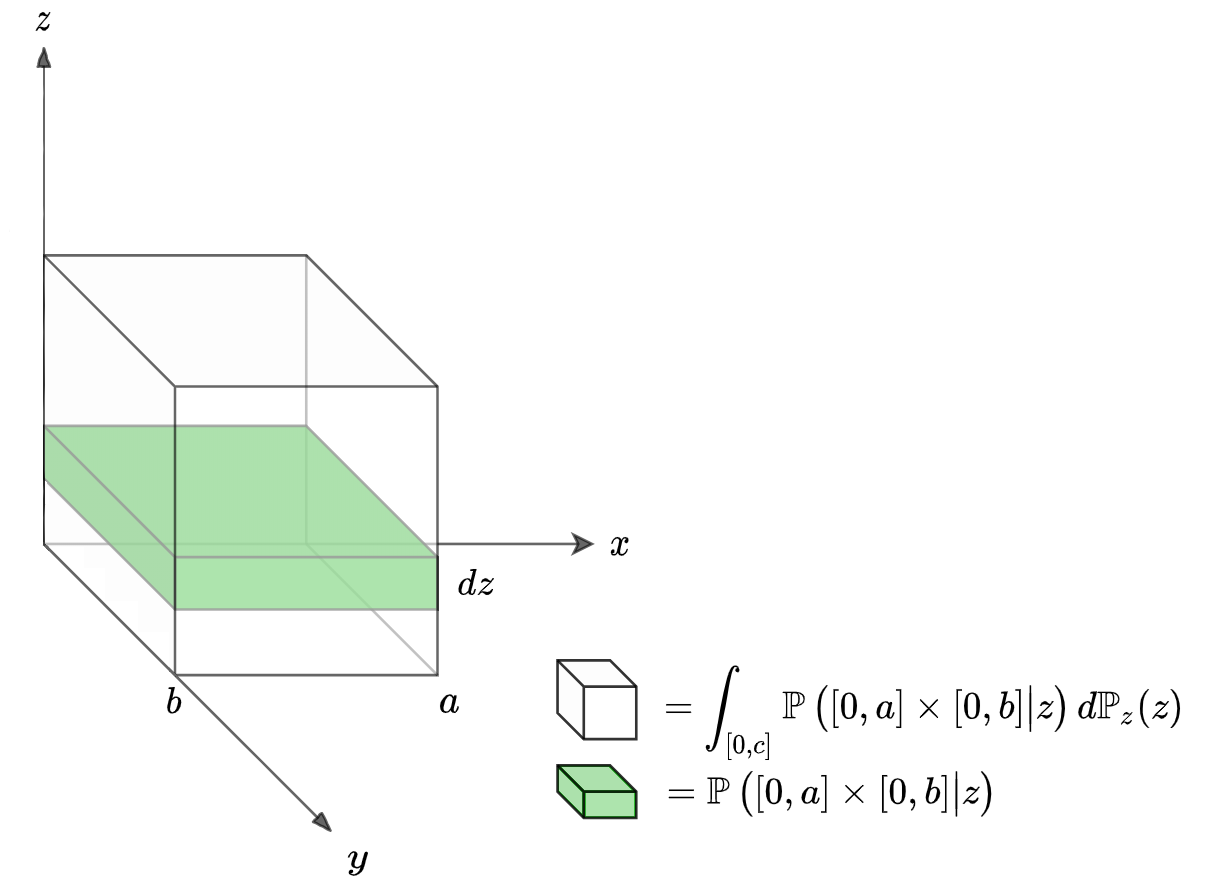
\includegraphics[scale=0.5]{images/disint2.png}
    \caption{ One can see that its is possible to construct a conditional measure to calculate the size of the green rectangle, however under the joint measure such measure is $0$. The disintegration Theorem provides us with the construction of such conditional measure.}
    \label{fig:disintegration}
\end{figure}
\subsection{Disintegration Theorem and Conditional Measures}

In this section we will present the disintegration theorem in the context of probability measures. We will use this theorem to present a derivation for RN-derivative equivalent of the product rule.

\begin{theorem} (Disintegration Theorem , for continuous probability measures): 

For a probability space $(Z, \calB(Z) ,\P)$ where $Z$ is a product space: $Z = Z_x \times Z_y$ and:
\begin{itemize}
    \item  $Z_x \subseteq \R^d, Z_y \subseteq \R^{d'}$
    \item  $\pi_i: Z \rightarrow Z_i$ be a measurable function known as the canonical projection operator ( i.e. $\pi_x(z_x,z_y) = z_x$ and $\pi^{-1}(z_x) = \{y | \pi(z_x) = z\}$)
\end{itemize}
Then there exists a measure $\P_{y|x}(\cdot | \vx)$ such that:
  \begin{align}
      \int_{Z_x \times Z_y} f(\vx, \vy) d\P(\vy) = \int_{Z_x}\int_{Z_y} f(\vx,\vy) d\P_{y|x}(\vy | \vx) d\P(\pi^{-1}(\vx)),
  \end{align}
 where $P_x(\cdot) = \P(\pi^{-1}(\cdot))$  is a probability measure typically refered to as a pullback measure and corresponds to the marginal distribution.
\end{theorem}

A direct consequence of the above instance of the disintegration theorem is the following, let $f(\vx,\vy) = \ind_{A_x \times A_y}(\vx,\vy)$:
\begin{align}
    \P(A_x \times A_y) = \int_{A_x}\P(A_y | \vx) d\P_x(\vx) 
\end{align}
 We can see that in the context of probability measures the above is effectively an analogue to the product rule 

We now have the required ingredients to show the following:
\begin{lemma}\label{lemma:rn_des}( RN-derivative product rule)
Given two probability measures defined on the same product space,  $(Z_x \times Z_y, \calB(Z_x \times Z_y) ,\P)$ and $(Z_x \times Z_y, \calB(Z_x \times Z_y) ,\Q)$, the Radon–Nikodym $\frac{d\P}{d\Q} (\vx,\vy)$ derivative can be decomposed as:
\begin{align}
    \frac{d\P}{d\Q} (\vx,\vy) = \frac{d\P_{y|x}}{d\Q_{y|x}}(\vy)\frac{d\P_x}{d\Q_x}(\vx)
\end{align}
\end{lemma}
\begin{proof}

Starting from:
\begin{align*}
    \P(A_x \times A_y) =  \int_{A_x}\P(A_y | \vx)  d\P_{x}(\vx) 
\end{align*}
We apply the Radon-Nikodym Theorem to $\P(A_y | \vx)$ and then to $P_x$:
\begin{align*}
    \P(A_x \times A_y) &=  \int_{A_x}\int_{A_y} \frac{d\P_{y|x}}{d\Q_{y|x}}(\vy) d\Q_{y|x}(\vy) d\P_{x}(\vx) \\
     &= \int_{A_x}\left(\int_{A_y} \frac{d\P_{y|x}}{d\Q_{y|x}}(\vy) d\Q_{y|x}(\vy)\right) \frac{d\P_{x}}{d\Q_{x}}(\vx)d\Q_{x}(\vx) \\
      &= \int_{A_x}\int_{A_y}\frac{d\P_{x}}{d\Q_{x}}(\vx)\frac{d\P_{y|x}}{d\Q_{y|x}}(\vy) d\Q_{y|x}(\vy) d\Q_{x}(\vx)
\end{align*}
Now  via the dissintegration we have that:
\begin{align*}
  \int_{A_x \times A_y} \frac{d\P_{x}}{d\Q_{x}}(\vx)\frac{d\P_{y|x}}{d\Q_{y|x}}(\vy) d\Q(\vx,\vy) = \int_{A_x}\int_{A_y}\frac{d\P_{x}}{d\Q_{x}}(\vx)\frac{d\P_{y|x}}{d\Q_{y|x}}(\vy) d\Q_{y|x}(\vy) d\Q_{x}(\vx)
\end{align*}
Thus we conclude that:
\begin{align*}
    \P(A_x \times A_y) = \int_{A_x \times A_y} \frac{d\P_{x}}{d\Q_{x}}(\vx)\frac{d\P_{y|x}}{d\Q_{y|x}}(\vy) d\Q(\vx,\vy), 
\end{align*}
which via the Radon-Nikodym Theorem imlpies:
\begin{align*}
    \frac{d\P}{d\Q} (\vx,\vy) = \frac{d\P_{y|x}}{d\Q_{y|x}}(\vy)\frac{d\P_x}{d\Q_x}(\vx).
\end{align*}
\end{proof}
The above result is used across a variety of different texts in stochastic processes, nonetheless it has proven difficult to find a resource for it and its derivation. We searched through a variety of graduate courses and books on measure and integration and could not find this result neither stated nor derived thus we decided it would be instructive to provide a sketch proof for it, since we will be using it multiple times.


\subsection{RN-Derivative of Itô-Processes}


As we hinted earlier Itô-processes don't admit a PDF since they are note absolutely continuous with respect to the Lebesgue measure. However some Itô-processes are absolutely continuous with respect to one another and thus we are able to compute their RN-derivatives which is useful if we want to compute the KL-divergence between the two processes.  First we must introduce the following notation:
\begin{definition} (Path Measure)
    For an Itô-process of the form:
    \begin{align*}
        d\rvx(t) = \rvb(t) + \rvsigma(t) d\rvw(t)
    \end{align*}
    defined in $[0,T]$. We call $\P$ the path measure of the above process whose outcome space $\Omega=C([0,T], \R^d)$ if the distribution $\P$ describes a weak solution to the above SDE \footnote{Weak solution is a terminology for a solution of an SDE that does not take into account an initial value problem.} to the above SDE.
\end{definition}

In short the path measure represents the probability measure associated to the stochastic process specified by the SDE. 

Now we can go ahead and present the following Theorem \citep{sarkka2019applied}:
\begin{theorem}\label{thrm:ito_ratio}\citep{sarkka2019applied}
Given two Itô-processes with the same constant volatility: 
    \begin{align*}
        d\rvx(t) = \rvb_1(t) + \sigma \rvw(t) \quad \rvx = \rvx_0\\
        d\rvy(t) = \rvb_2(t) + \sigma\rvw(t) \quad \rvy = \rvx_0
    \end{align*}
The RN-Derivative of their respective path measures $\P,\Q$ is given by:
\begin{align} \label{eq:girsanov}
    \frac{d\P}{d\Q}(\cdot) = \exp\left(-\frac{1}{2\sigma^2}\int_0^t ||\rvb_1(s) - \rvb_2(s)||^2 ds + \frac{1}{\sigma^2}\int_0^t (\rvb_1(s) - \rvb_2(s))^{\top}d\rvw(s) \right)
\end{align}
\end{theorem}
Note that in the case where we take the RN-derivative with respect to Brownian motion (i.e. $\rvb_2(t) =0, \; \sigma=1$), we have the following expression:
\begin{align} \label{eq:girsanov_0}
    \frac{d\P}{d\W}(\cdot) = \exp\left(-\frac{1}{2}\int_0^t ||\rvb_1(s) ||^2 ds + \int_0^t \rvb_1(s)^{\top}d\rvw(s) \right),
\end{align}
which is popularly refered to as Girsanov's theorem as it is one of the main elements in said theorem.
%\chapter{Background} 
\chapter{The Schrödinger Bridge Problem}

As originally posed by Schrödinger in \citep{schrodinger1931uber, schrodinger1932theorie} the Schrödinger Bridge consists in finding a posterior stochastic evolution between two distributions that is optimally close to a Brownian motion prior in a KL sense:
\begin{align} \label{eq:schrobirdge}
    \hat{\Q}= \argmin_{\Q \in \calD(\pi_0, \pi_1)} \KL\left(\Q \big|\big| \W\right),
\end{align}
where:
\begin{align} \label{eq:kl_sho}
    \ \KL\left(\Q \big|\big| \W\right) = \E_{\Q}\left[\ln \frac{d\Q}{d\W}\right].
\end{align}
To the eye of a probabilistic modeller this objective may be initially quite confusing.  Mainly because it is minimising the KL divergence between a "posterior" distribution $\Q$ and a "prior" distribution $\W$ which does not match the usual variational inference objectives that arise from minimising an Evidence Lower Bound. In order to give a sound interpretation to the objective in Equation \ref{eq:schrobirdge} we will look into the Schrödinger Bridge's formulation as a rare event and additionally comment on the maximum entropy like nature of the objective.

\section{Rare Events and Maximum Entropy }

First let our sample space be the space of random functions with the unit interval as pre-image $C([0,1], \R^d)$ that is a sample  represents a function of the form $\vx : [0, 1]:  \rightarrow \R^d$.  We now take a set of i.i.d samples $\{\rvx_{i}(t)\}_{i=1}^N$ following standard Brownian motion defined on $C([0,1], \R^d)$. The empirical distribution for $\{\rvx_{i}(t)\}_{i=1}^N$ is the defined by:
\begin{align}\label{eq:empirical}
    \hat{\W}(A) = \frac{1}{N}\sum_{i=1}^N \ind\left(\rvx_i(t) \in A\right)  , \quad A \in \calB(\R^d)^{[0,1]},
\end{align}
then we might want to ask what is the probability that the empirical distribution prescribes marginals $\pi_0, \pi_1$ which cannot be attained by Brownian motion:
\begin{align}
    {P}\left(\hat{\W} \in \mathcal{D}(\pi_0, \pi_1) \right)
\end{align}
it turns out that result from the theory of large deviations (Sanov's Theorem) allows us to compute an asymptotic expression for such probability:
\begin{align} \label{eq:max_ent}
    {P}\left(\hat{\W} \in \mathcal{D}(\pi_0, \pi_1) \right) \sim \exp\left(-N\inf_{\Q \in \calD(\pi_0, \pi_1)} \!\!\!\!\!\KL\left(\Q \big|\big| \W\right)\right).
\end{align}
For a more technically thorough introduction please check \cite{leonard2013survey}. Note that the exponent for the probability in Equation \ref{eq:max_ent} extremises the KL-divergence following the Principle of Minimum Discrimination Information by \cite{kullback1997information} which is a generalisation of Edwin Jane's Maximum Entropy Principle \citep{jaynes1957information,jaynes2003probability} to continuous distributions. Note one can observe the connection between maximising entropy and minimising KL divergence by considering the discrete setting where minimising KL divergence with respect to a uniform reference distribution is equivalent to maximising entropy. In simple words we are selecting a distribution $\hat{\Q}$ subject to the marginal constraints that is as close as possible given prior knowledge $\W$.

\section{Dynamic Formulation}
The Dynamic formulation of the Schrödinger follows directly from the exponent in the maximum entropy formulation.  The dynamic version of the Schrödinger bridge is written in terms of path measures that describe the stochastic dynamics defined over the unit interval.
\begin{definition}
    (Dynamic Schrödinger Problem) The dynamic Schrödinger problem is given by:
    \begin{align}
        \inf_{\Q \in \calD(\pi_0, \pi_1)} \KL\left(\Q \big|\big| \W^{\gamma}\right)
    \end{align}
    Where $\Q \in \calD(\pi_0, \pi_1)$ is a path measure with prescribed marginals of $\pi_0, \pi_1$ at times $0, 1$ and $\W_{\gamma}$ is the Wiener measure with volatility $\gamma$. 
\end{definition}
\subsection{As a Stochastic Control Problem}

The two results presented below are from \cite{pavon1991free}. For Pedagogical reasons we provide a proof sketch of these two results.

We can represent $\Q$ as the distribution which evolves according to the solution of an SDE of the form:
\begin{align*}
    d\rvx(t) = \rvb^{+}(t) dt + \sqrt{\gamma} \rvw(t)
\end{align*}
\begin{lemma}\citep{pavon1991free}
    The KL Divegence between $\Q$ and $\W_{\gamma}$ can be decomposed as:
\begin{align}\label{eq:free_energy_1}
     \KL\left(\Q \big|\big| \W^{\gamma}\right) = \KL(\pi^{\Q}_0 || \pi_0) + \E_\Q\left[\int_0^1 \frac{1}{2\gamma}\big|\big|\rvb^{+}(t) \big|\big|^2 dt\right]
\end{align}
\end{lemma}
\begin{proof}
Via the Disintegration theorem and Theorem \ref{lemma:rn_des} we can condition on the endpoint and re-write the RN derivative as:
\begin{align*}
    \frac{d\Q}{d\W} = \frac{\pi_0^\Q}{\pi_0} \frac{d\Q_{(0,1]}}{d\W_{(0,1]}}\left(\cdot | \rvx(0) =\vx\right)
\end{align*}
where the disintegration $\Q_{(0,1]}\left(\cdot | \rvx(0) = \vx \right)$ is a solution $d\rvx(t) = \rvb_t dt + \gamma \rvw(t), \; \rvx(0) \sim \pi_0^\Q$ then by Theorem \ref{thrm:ito_ratio} we can express the RN-derivative in terms of  drift $\vb(\rvx(t), t)$:
\begin{align*}
    \frac{d\Q}{d\W} = \frac{\pi_0^\Q}{\pi_0}\exp\left(\int_0^1\frac{1}{2\gamma} \big|\big|\rvb^+(t)\big|\big|^2 dt\right),
\end{align*}
Now substituting the above back into the KL divergence completes the result for Theorem \ref{eq:free_energy_1}.
\end{proof}
Now we can equivalently express $\Q$ as the solution to a reverse time diffusion :
\begin{align}
    d\rvx(t) = \rvb^{-}(t) dt + \sqrt{\gamma} \rvw^{-}(t), 
\end{align}
where $\rvx(t)$ is adapted to the reverse filtration $(\calF^{-}_i)_{i\in T}$ that is $\calF^{-}_t \subseteq \calF^{-}_s \; s \leq t $ \footnote{As mentioned before this just means $\rvx(t)$  is only aware about the future}.  Where:
\begin{align}\label{eq:nelson}
    {\rvb^{+}(t) - \rvb^{-}(t)} =\gamma \nabla_{\vx} p(\rvx(t), t).
\end{align}
Where $p(\rvx(t), t)$ is the solution to the FPK equation. The above is typically known as Nelson's duality equation and it relates the forwards drift to the dual backwards drift \citep{nelson1967dynamical}. 

Using reverse diffusion \cite{pavon1991free} decompose the KL divergence as done with the forward diffusion:
\begin{lemma}\label{lemma:control}\citep{pavon1991free}
    The KL Divegence between $\Q$ and $\W_{\gamma}$ can be decomposed as:
\begin{align}\label{eq:free_energy_2}
     \KL\left(\Q \big|\big| \W^{\gamma}\right) = \KL(\pi^{\Q}_1 || \pi_1) + \E_\Q\left[\int_0^1\frac{1}{2\gamma} \big|\big|\rvb^{-}(t)\big|\big|^2 dt\right]
\end{align}
\end{lemma}
Then using the drift based formulations defined above \cite{pavon1991free} derive alternate (yet equivalent) objectives for the Schrödinger Bridge objective:

\begin{itemize}
\item Forward Objective: 
\begin{align} \label{eq:controlled_bridge_forward}
    \min_{\Q \in \calD(\pi_0, \pi_1)} \KL\big(\Q \big|\big| \W^{\gamma}\big)& = \min_{\rvb^{+} \in \calB }  \E_\Q\left[\int_0^1 \frac{1}{2\gamma}\big|\big|\rvb^{+}(t) \big|\big|^2 dt\right] \nonumber \\
    s.t.\;\;\; d\rvx(t) = \rvb^{-}(t) &dt + \sqrt{\gamma} \rvw(t), \;\; \rvx(0) \sim \pi_0, \;\; \rvx(1) \sim \pi_1
\end{align}
\item Backward Objective
\begin{align} \label{eq:controlled_bridge_backward}
    \min_{\Q \in \calD(\pi_0, \pi_1)} \KL\big(\Q \big|\big| \W^{\gamma}\big)& = \min_{\rvb^{-} \in \calB }  \E_\Q\left[\int_0^1 \frac{1}{2\gamma}\big|\big|\rvb^{-}(t) \big|\big|^2 dt\right] \nonumber \\
    s.t.\;\;\; d\rvx(t) = \rvb^{+}(t) &dt + \sqrt{\gamma} \rvw^{-}(t), \;\; \rvx(1) \sim \pi_1 , \;\; \rvx(0) \sim \pi_0
\end{align}.
\end{itemize}
Notice that the conditioning carried out by the Disintegration theorem allows us to remove one of the boundary constraints and integrate it as an initial value problem to the objective. This result is what inspired us the most in the design of an iterative algorithm for solving finding the Schrödinger Bridge numerically. 
\section{Static Formulation}
\begin{definition}\label{def:static_bridge}
    (Static Schrödinger Problem) The static Schrödinger bridge consists in finding the joint distribution $q(\vx, \vy) \in \calD(\pi_0(\vx), \pi_1(\vy))$ which is closest to the Brownian motion prior, subject to marginal constraints, that is :
    \begin{align}\label{eq:static_bridge}
        \inf_{q(\vx,\vy)} \KL (q(\vx,\vy)  &|| p^{\W^{\gamma}}(\vx,\vy)) \nonumber \\
        s.t. \;\;\; \pi_0(\vx) = \int q(\vx,\vy) d\vy, &\;\;\pi_1(\vy) = \int q(\vx,\vy) d\vx,
    \end{align}
\end{definition}
we will know illustrate how this result is arrived to from the dynamic version. Most surveys and paper relating the Schrödinger include some form of the derivation that we are about to present, however they skip several steps which may make it inaccessible to a more applied community. 
\begin{theorem}\citep{follmer1988random}
    The dynamic Schrödinger bridge is solved by :
\begin{align}
    \Q^{*} (\cdot) =  \int \W^{\gamma} \left(\cdot | \vx, \vy\right)  q^{*}(\vx,\vy) d\vx d\vy 
\end{align}
    where $q^*$ is the optimal density that solves the static bridge:
    \begin{align*}
        q^{*}(\vx,\vy)& = \arginf_{q(\vx,\vy)} \KL (q(\vx,\vy)  || p^{\W^{\gamma}}(\vx,\vy))  \\
        s.t. \;\;\; \pi_0(\vx) &= \int q(\vx,\vy) d\vy, \;\;\pi_1(\vy) = \int q(\vx,\vy) d\vx,
    \end{align*}
    and :
    \begin{align*}
        \W^{\gamma} \left(\cdot | \vx, \vy\right)  = \W_{(0,1)}^{\gamma}\left(\cdot | \rvx(0) =\vx, \rvx(1) =\vy\right),
    \end{align*}
    Is the conditional (disintegration) of the Wiener measure about its endpoints.
\end{theorem} %\vspace{-0.6cm}
\begin{proof}
Firstly we decompose the KL divergence over path measures $\KL\left(\Q \big|\big| \W\right)$ using Lemma \ref{lemma:rn_des}, conditioning on the endpoints $\rvx(0), \rvx(1)$ we can re-express the RN-derivative as:
\begin{align}
    \frac{d\Q}{d\W} = \frac{q(\vx, \vy)}{p^{\W^{\gamma}}(\vx. \vy)}\frac{d\Q_{(0,1)}}{d\W_{(0,1)}}\left(\cdot | \rvx(0) =\vx, \rvx(1) =\vy\right)
\end{align}
Let $\Q_{(0,1)}(\cdot |  \rvx(0) =\vx, \rvx(1) =\vy) = \Q(\cdot |  \vx,\vy)$. Substituting the above decomposition back into the KL divergnece and marginalising where possible we arrive at: 
\begin{align} \label{eq:follmer_kl}
    \KL\left(\Q \big|\big| \W\right) =&  \KL\left(q(\vx, \vy) \big|\big| p^{\W^{\gamma}}(\vx. \vy) \right)  + \E_{\Q}\left[\frac{d\Q}{d\W^\gamma}\left(\cdot | \vx, \vy\right)\right], \nonumber \\
    =&  \KL\left(q(\vx, \vy) \big|\big| p^{\W^{\gamma}}(\vx. \vy) \right)  + \E_{q(\vx,\vy)}\left[\KL\left(\Q(\cdot |  \vx,\vy)\big|\big|\W^{\gamma}(\cdot |  \vx,\vy)\right)\right].
\end{align}
Now notice that the conditional $\Q_{(0,1)}(\cdot |  \rvx(0) =\vx, \rvx(1) =\vy)$ is not affected by the boundary constraints thus we can set $\Q(\cdot | \vx,\vy) = \W^\gamma\left(\cdot | \vx, \vy\right)$ making the second term 0, and leaving us with the static bridge. It then suffices to reverse the Disintegration theorem in order to build up $\Q^{*}$ from $q^{*}$ and $\Q^{*}(\cdot | \vx,\vy)$ completing the proof.
\end{proof}

The earliest references we found for the above result are given by \cite{follmer1988random}, where the decomposition of the KL divergence for two diffusion's (Equation \ref{eq:follmer_kl}) is provided. However we were not able to find a good reference for Lemma \ref{lemma:rn_des} and thus we have provided an instructive derivation for it.
\subsection{As an Entropy Regularised Optimal Transport Problem}

Here we will present and discuss a very well studied \citep{mikami2008optimal,leonard2012schrodinger,leonard2013survey,carlier2017convergence} connection between the static bridge and the Wasserstein distance.  Using that for the Wiener process $\W^\gamma$ prior we have :
\begin{align}
    p^{\W^{\gamma}}(\vx,\vy) = p^{\W^{\gamma}}_0(\vx)\calN(\vy | \vx, \sqrt{\gamma}\I)
\end{align}
and that the term:
\begin{align*}
    \int q(\vx, \vy)\ln  p^{\W^{\gamma}}_0(\vx) d\vx d\vy =  \int \pi_0(\vx) \ln  p^{\W^{\gamma}}_0(\vx) d\vx  
\end{align*}
does not depend on $q$ (due to the constraints). Substituting the above into Equation \ref{eq:static_bridge} we arrive at:
\begin{align}
    &\inf _{q \in \calD(\pi_0, \pi_1)}\int \int -\frac{||\vx - \vy ||^2}{2\gamma} q(\vx, \vy) d\vx d\vy  + \int \int q(\vx, \vy) \ln q(\vx, \vy) d\vx d\vy \nonumber \\
    &=\inf _{q \in \calD(\pi_0, \pi_1)}\int \int -\frac{||\vx - \vy ||^2}{2} q(\vx, \vy) d\vx d\vy  - \gamma \text{H} \left(q(\vx, \vy)\right)
\end{align}
which is an entropy regularised optimal mass transport problem (OMT) \citep{villani2003topics} with a quadratic cost function. Furthermore as the volatility/noise of the Brownian motion prior goes to 0 ($\gamma \downarrow 0$) the above quantity converges to $\calW^2_{2}(\pi_0, \pi_1)$ (Squared Wasserstein distance in an $L_2$ metric space).
\subsection{The Schrödinger System}

Following \cite{pavon2018data} Lagrangian of Equation \ref{eq:static_bridge} is given by :
\begin{align}\label{eq:schro_lagrangian}
    \calL(q, \lambda,  \mu) &=  \KL (q(\vx,\vy)  || p^{\W^{\gamma}}(\vx,\vy))  \nonumber\\
    &+ \int \lambda(\vx)\left( \int q(\vx,\vy)d\vy -\pi_0(\vx)\right)d\vx \nonumber \\
    &+ \int \mu(\vy) \left(\int q(\vx,\vy) d\vx - \pi_1(\vy)\right) d\vy
\end{align}
Let $p^{\W^{\gamma}}(\vx,\vy) = p^{\W^{\gamma}}_0(\vx)p^{\W^{\gamma}}(\vy|\vx)$. Where $p^{\W^{\gamma}}_0(\vx)$ is the marginal prior which we are free to set and $p^{\W^{\gamma}}(\vy|\vx)=\calN(\vy | \vx, \sqrt{\gamma}\I)$ is the transition density of the prior. Then we set functional derivative $\frac{\delta \calL}{\delta q(\vx, \vy)}$ to 0 and obtain:
\begin{align*}
    1 + \ln q(\vx, \vy)  - \ln p^{\W^{\gamma}}(\vy|\vx)
    - \ln p^{\W^{\gamma}}_0(\vx)+ \lambda(\vx)
+ \mu(\vy) = 0, \nonumber
\end{align*}
rearranging:
\begin{align*}
{q^{*}(\vx, \vy) }  = \exp\left(  \ln p^{\W^{\gamma}}_0(\vx) -\lambda(\vx) -1\right)p^{\W^{\gamma}}(\vy|\vx)\exp\left(- \mu(\vy)\right) \nonumber
\end{align*}
which we can re-express in terms of the auxiliary potentials $\hphi_0(\vx), \phi_1(\vy)$:
\begin{align*}
{q^{*}(\vx, \vy) }  = \hphi_0(\vx)p^{\W^{\gamma}}(\vy|\vx)\phi_1(\vy), \nonumber
\end{align*}
satisfying:
\begin{align}
    \hphi_0(\vx) \int \phi_1(\vy) p^{\W^{\gamma}}(\vy|\vx) d\vy = \pi_0(\vx)  \nonumber\\ 
    \phi_1(\vy) \int \hphi_0(\vx) p^{\W^{\gamma}}(\vy|\vx) d\vx = \pi_1(\vy), \nonumber
\end{align}
where we re-lable the terms with the integrals to:
\begin{align}
    \phi_0(\vx) &= \int \phi_1(\vy) p^{\W^{\gamma}}(\vy|\vx) d\vy \nonumber\\ 
    \hphi_1(\vy) &= \int \hphi_0(\vx) p^{\W^{\gamma}}(\vy|\vx) d\vx. \nonumber
\end{align}
Placing it all together, the following linear functional system is known as the Schrödinger system:
\begin{align}
    \hphi_0(\vx) \phi_1(\vx)  = \pi_0(\vx)  \nonumber \\ 
    \hphi_1(\vx) \phi_1(\vy)  = \pi_1(\vy).
\end{align}
To obtain the distribution $\pi^{*}_t(\vz)$ (Solution to the FPK equation for the optimal $Q^{*}$) :
\begin{align}
    \pi^{*}_t(\vz) =  \hphi_t(\vz) \phi_t(\vz) 
\end{align}
where:
\begin{align}
    \phi_t(\vz) &= \int \phi_1(\vy(1) ) p^{\W^{\gamma}}(\vy(1)|\vz(t)) d\vy(1) \nonumber\\ 
    \hphi_t(\vz) &= \int \hphi_0(\vx(0)) p^{\W^{\gamma}}(\vz(t)|\vx(0)) d\vx(0). \nonumber
\end{align}
Note that by Proposition 3.3 of \cite{pavon1991free} the optimal control signal/drift $\rvb_t^+$ can be recoverd from the solution of the Schrödinger system:
\begin{align} \label{eq:drifr_potential}
    \rvb_t^{+} = \gamma \nabla \ln \phi_t(\vx(t) )
\end{align}
\section{Half Bridges}

The half bridge problem as presented in \cite{pavon2018data} is a simpler variant of the full Schrödinger bridge with only one boundary constraint. 

\begin{definition}
The forward half bridge is given by:
    \begin{align}
        {\Q}^{*} = \inf_{\Q  \in \calD(\pi_0, \cdot)} \KL (\Q || \W) 
    \end{align}
\end{definition}
\begin{theorem}\label{thrm:half_bridge_forward}
    The forward half bridge admits the following solution: 
\begin{align}
    {\Q}^{*}\left(A_0 \times A_{(0,1]}\right) =  \int_{A_0\times A_{(0,1]}} \frac{d \pi_0}{ dp_0^\W} d\W
\end{align}
\end{theorem}
\begin{proof}
Via the disintegration theorem we have the following decomposition of KL
\begin{align}
    \KL(\Q || \W) = \KL(p|| \pi_0 )  + \E_p\left[\KL(\Q(\cdot| \vx) || \W(\cdot | \vx))\right] \nonumber
\end{align}
Thus via matching the terms accordingly we can construct $\hat{P}$ to set the second term to $0$ and match the constraints:
\begin{align}
    {\Q}^{*}\left(A_0 \times A_{(0,1]}\right) = \int_{A_0 \times A_{(0,1]}}\!\!\!\!\!\!\!\!\!\!\!\!\W(A_{(0,1]} | \vx) d\pi_0(\vx)
\end{align}
\begin{align}
    {\Q}^{*} &= \int_{A_0}  \frac{d\pi_0}{dp_0^\W}(\vx)   \W(\cdot | \vx) d p^\W(\vx) \nonumber \\
    &= \int_{A_0 \times A_{(0,1]} }  \frac{d\pi_0}{dp_0^\W}(\vx)  d \W
\end{align}
\end{proof}
\begin{definition}
The backwards half bridge is given by:
    \begin{align}
        {\P}^{*} = \inf_{\Q  \in \calD(\cdot, \pi_1)} \KL (\P || \W) 
    \end{align}
\end{definition}
\begin{theorem}\label{thrm:half_bridge_backward}
     The backward half bridge admits the following solution: 
\begin{align}
    {\P}^{*}\left( A_{[0,1)} \times A_1\right) =  \int_{ A_{[0,1)} \times A_1}  \frac{d \pi_1}{ d p_1^\W} d\W
\end{align}

\end{theorem}
\begin{proof}
Same as Theorem \ref{thrm:half_bridge_forward}.
\end{proof}


Note how the main difference between the full and half bridges is that the half bridges admit a closed form solution in terms of known quantities. Similarly to the full bridge the half bridges admit a static formulation:

\begin{definition}
The static forward bridge is given by the following objective
 \begin{align}\label{eq:static_bridge_forward}
        \inf_{q(\vx,\vy)} \KL  &(q(\vx,\vy) || p^{\W^{\gamma}}(\vx,\vy)) \nonumber \\
        s.t. \;\;\;& \pi_0(\vx) = \int q(\vx,\vy) d\vy, 
\end{align}
\end{definition}
\begin{theorem}\label{thrm:static_half_forward}
     The static forward bridge admits the following solution:
     \begin{align}
         q^{*}(\vx,\vy) = p^{\W_{\gamma}}(\vx, \vy)\frac{\pi_0(\vx)}{p^{\W_{\gamma}}(\vx)}
     \end{align}
\end{theorem}
\begin{proof}
See \cite{pavon2018data} for the solution of the backward half bridge. Proof is simple and easy to adapt to the forward bridge. 
\end{proof}
\begin{definition}
The static backward bridge is given by the following objective
 \begin{align}\label{eq:static_bridge_backward}
        \inf_{p(\vx,\vy)} \KL  &(p(\vx,\vy) || p^{\W^{\gamma}}(\vx,\vy)) \nonumber \\
        s.t. \;\;\;& \pi_1(\vy) = \int p(\vx,\vy) d\vx, 
\end{align}
\end{definition}
\begin{theorem}\label{thrm:static_half_backward}
     The static backwards bridge admits the following solution:
     \begin{align}
         p^{*}(\vx,\vy) = p^{\W_{\gamma}}(\vx, \vy)\frac{\pi_1(\vy)}{p^{\W_{\gamma}}(\vy)}
     \end{align}
\end{theorem}
\begin{proof}
See \cite{pavon2018data}.
\end{proof}


%\chapter{Algorithmic Framework} 
\chapter{Iterative Proportional Fitting Procedure}

So far we have introduced the Schrödinger bridge problem as well as its simpler half bridge variants. We have also introduced the Schrödinger system and loosely hinted at a potential iterative solution, nonetheless we have not yet presented a full solution and discussed its guarantees / properties.

In this chapter we will be studying an algorithmic framework known as the Iterative Proportional Fitting Procedure (IPFP) \citep{csiszar1975divergence, kullback1968probability, ruschendorf1995convergence,cramer2000probability} and describe its usage for solving the Schrödinger bridge. Furthermore we will formalise a previously made observation that connects Fortet's Iterative scheme \citep{fortet1940resolution} for solving the Schrödinger system with the more general IPFP . 

\section{Fortet's Algorithm}

Firstly let us start by introducing Fortet's algorithm, which is probably the oldest algorithm with a proof of convergence \cite{fortet1940resolution} for solving the Schrödinger system.

\begin{algorithm} \label{alg:fortet}
\SetKwInOut{Input}{input}
\Input{$\pi_0(\vx), \pi_1(\vy), p(\vy | \vx)$}
Initialise $\phi_0^{(0)}(\vx)$ such that $\phi_0^{(0)}(\vx) <\!< \pi_0(\vx)$ \\
    \Repeat{convergence}{
      $\hphi_0^{(i)}(\vx) := \frac{\pi_0(\vx)}{\phi_0^{(i)}(\vx)}$ \\
      $\hphi_1^{(i)}(\vy) := \int  p(\vy | \vx) \hphi_0^{(i)}(\vx) d\vx$ \\
      $\phi_1^{(i)}(\vy) := \frac{\pi_1(\vy)}{\hphi_1^{(i)}(\vy)}$ \\
      $\phi^{(i+1)}_0(\vx) := \int  p(\vy | \vx) \phi_1^{(i)}(\vy) d\vy$\\
      $i:=i+1$
    }
\Return{$\hphi_0^{(i)}(\vx), \phi_1^{(i)}(\vy)$}
\caption{Fortet's Iterative Procedure}
\end{algorithm}
Modern adaptations for the proof of convergence for the Algorithm  \ref{alg:fortet} can be found in \citep{essid2019traversing, chen2016entropic}, however these proofs are very technical and beyond the scope of this survey.  Let us now provide an intuition behind each step in the algorithm :

\begin{itemize}
    \item $\hphi_0^{(i)}(\vx) := \frac{\pi_0(\vx)}{\phi_0^{(i)}(\vx)}$: enforces the marginal/boundary constraint at time $0$. That is it enforces that the product of the factors/potentials match the marginal distribution $\pi_0$ for a given 
    \item $\hphi_1^{(i)}(\vy) := \int  p(\vy | \vx) \hphi_0^{(i)}(\vx) d\vx$ : Now that we have the factors $\phi_0^{(i)}(\vx) \hphi_0^{(i)}(\vx) := {\pi_0(\vx)}$ for the marginal at $t=0$ we transport/transition them to the marginal at time $t=1$ via marginalising the current estimate of the joint posterior $\pi_1(\vy) = \phi_1(\vy) \int p(\vy| \vx) \hphi_0^{(i)}(\vx) d\vx$.
    \item  $\phi_1^{(i)}(\vy) := \frac{\pi_1(\vy)}{\hphi_1^{(i)}(\vy)}$: As with $t=0$ we enforce the marginal/boundary  constraint such that  $\phi_1^{(i)}(\vy) \hphi_1^{(i)}(\vy) := {\pi_1(\vy)}$. 
    \item $\phi^{(i+1)}_0(\vx) := \int  p(\vy | \vx) \phi_1^{(i)}(\vy) d\vy$; Now that we have enforced the constraint for $t=1$ we marginalise our current estimate of the joint to move from $\vy$ to $\vx$ and repeat.
\end{itemize}

Now we can see that Fortet's algorithm is quite intuitive, we initialise the potential at time $t=0$ and what is effectively the prior marginal and iterate the Schrödinger system until reaching a fixed point where the constraints are satisfied by alternating the constraint satisfaction between $t=0$ and $t=1$, the leads us to make the following observation:
\begin{observation}
Fortet's algorithm starting at $t=1$ rather than $t=0$ is equivalent sequentially alternating between solving  Forwards and Backwards static Half Bridges.
\begin{algorithm} \label{alg:ipfp_intro}
\SetKwInOut{Input}{input}
\Input{$\pi_0(\vx), \pi_1(\vy), p(\vy | \vx)$}
Initialise:\\
$p^{\W^{\gamma}}_1(\vy)$ such that $p^{\W^{\gamma}}_1(\vy) <\!< \pi_1(\vy)$ \\
$ q^{*}_{0}(\vx,\vy) =p^{\W^{\gamma}}(\vx,\vy)$\\
$i=0$ \\
    \Repeat{convergence}{
      $i := i + 1$ \\
     $ p^{*}_{i}(\vx,\vy) = \inf_{p(\vx,\vy) \in \calD( \cdot, \pi_1)} \KL  (p(\vx,\vy) || p^{*}_{i-1}(\vx,\vy))$\\ 
     $ q{*}_{i}(\vx,\vy)  = \inf_{q(\vx,\vy) \in \calD(\pi_0, \cdot)} \KL  (q(\vx,\vy) ||  p^{*}_{i}(\vx,\vy))$
    }
\Return{$q^{*}_{i}(\vx,\vy) , p{*}_{i}(\vx,\vy)$}
\caption{Alternating half bridges (\cite{kullback1968probability} IPFP) }
\end{algorithm}
\end{observation}
\begin{proof}
Consider the first two iterations of Algorithm \ref{alg:ipfp_intro}:

Using Theorem \ref{thrm:static_half_backward}  The solution to the Backward half bridge
 \begin{align}
        \inf_{p(\vx,\vy) \in \calD( \cdot, \pi_1)} \KL  &(p(\vx,\vy) || p^{\W^{\gamma}}(\vx,\vy)) \nonumber 
\end{align}
is:
\begin{align}
    p_0^{*} (\vx, \vy) = p^{\W^{\gamma}}_0(\vx) p^{\W^{\gamma}}(\vy| \vx) \frac{\pi_1(\vy)}{p^{\W^{\gamma}}_1(\vy)}
\end{align}
Now we setup the following forward bridge:
\begin{align}
    \arginf_{q_0(\vx, \vy)  \in \calD(\pi_0 , \cdot)}\KL (q_0(\vx, \vy) ||p_0^{*} (\vx, \vy))
\end{align}
which following theorem \ref{eq:static_bridge_forward} can be solved by:
\begingroup
\allowdisplaybreaks
\begin{align}
    q_0^{*} (\vx, \vy) &= p_0^{*} (\vx, \vy) \frac{\pi_0(\vx)}{p_0^{*} (\vx)} \\
 &=  p^{\W^{\gamma}}(\vy| \vx) \frac{\pi_1(\vy)}{p^{\W^{\gamma}}_1(\vy)} \frac{\pi_0(\vx)}{\int   p^{\W^{\gamma}}(\vy| \vx) \frac{\pi_1(\vy)}{p^{\W^{\gamma}}_1(\vy)} d\vy}
\end{align}
\endgroup

If we proceed on to the second iteration of this procedure the  following backward bridge step will yield:
\begin{align}
    p_1^{*} (\vx, \vy) =  q_0^{*} (\vx, \vy) \frac{p^{\W^{\gamma}}_1(\vy)}{ \underbrace{\displaystyle\int \frac{p^{\W^{\gamma}}(\vy| \vx)\pi_0(\vx)}{\int p^{\W^{\gamma}}(\vy| \vx) \frac{\pi_1(\vy)}{p^{\W^{\gamma}}_1(\vy)} d\vy}d\vx}_{{\phi}^{1}(\vy)}} 
\end{align}
and forward step:
\begin{align}
    q_1{*} (\vx, \vy) &= p_1^{*} (\vx, \vy) \frac{\int    p^{\W^{\gamma}}(\vy| \vx) \frac{\pi_1(\vy)}{p^{\W^{\gamma}}_1(\vy)}  d \vy}{\int    p^{\W^{\gamma}}(\vy| \vx) \frac{\pi_1(\vy)}{{\phi}^{1}(\vy)}  d \vy}
\end{align}
re-labeling: 
\begin{align}
    \phi^0(\vy)&=p^{\W^{\gamma}}_1(\vy) \\ 
    \hat{\phi}_0^{i}(\vx) &= \int  p^{\W^{\gamma}}(\vy| \vx) \frac{\pi_1(\vy)}{{\phi}^{i}(\vy)}  d \vy
\end{align}
we can make an inductive argument on $i$ for the following inductive hypothesis \footnote{Some simple term cancellation steps have been omitted to reduce verbosity.}:
\begin{align} \label{eq:recurrence}
  {\phi}^{i+1}(\vy) =  \displaystyle\int \frac{p^{\W^{\gamma}}(\vy| \vx)\pi_0(\vx)}{\int p^{\W^{\gamma}}(\vy| \vx) \frac{\pi_1(\vy)}{\phi^i(\vy)} d\vy}d\vx
 \end{align}
 \begin{align}
  p_i^{*} (\vx, \vy) =   q_{i-1}^{*} (\vx, \vy) \frac{\phi^{i-1}(\vy)}{{\phi}^{i}(\vy)} 
\end{align}
 \begin{align}
      q_i{*} (\vx, \vy) =     p_i^{*} (\vx, \vy) \frac{\hat{\phi}_0^{i-1}(\vx)}{\hat{\phi}_0^{i}(\vx)} 
\end{align}
We can see that the  recurrence in Equation \ref{eq:recurrence} is the exact same set of steps performed by Fortet's algorithm if we were to reverse the time order or start Fortet's algorithm at step 5 and consider the first steps  as an initialisation of $\phi_0(\vy)$.
\end{proof}

Whilst in hindsight the above observation may seem simple we regard it as a contribution nonetheless as we have not observed a formal argument made towards that connection. As we will see in the following sections this connections bridges the stream of iterative proportional fitting algorithms with Fortet's algorithm.

\section{Kullback's IPFP}
The original Iterative Proportional Fitting Procedure (IPFP) consists en estimating a normalised contingency table (discrete joint distribution) given prescribed marginals, via some form of information discrimination/maximum entropy principle. Our interest however is in the continuous variant of IPFP which dates back to Kullback \citep{kullback1968probability}.

What we call in this section Kullback's IPFP is in fact Algorithm \ref{alg:ipfp_intro} which we have introduced via its formal connection to Fortet's algorithm.  The first complete proof for convergence to the  Schrödinger bridge Algorithm \ref{alg:ipfp_intro} was provided in \cite{ruschendorf1995convergence} using information geometric arguments from \cite{csiszar1975divergence}.


\section{Generalised IPFP}

\begin{figure}[t!]
    \centering
    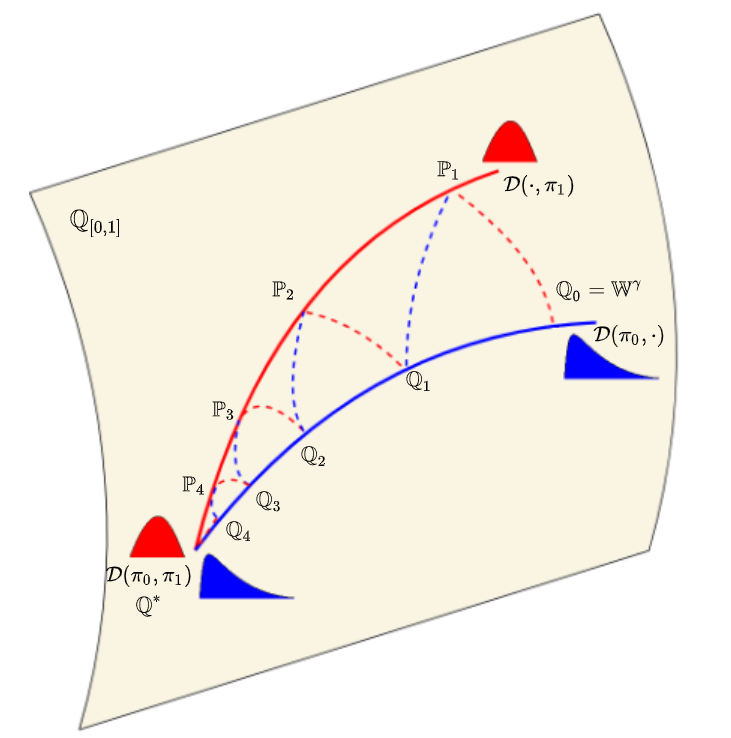
\includegraphics[]{images/g-IPFP_ready.PNG}
    \caption{Illustration of the iterative proportional fitting procedure, inspired and adapted from Figure 1 in \cite{bernton2019schr}. The red line represents valid Ito-process posteriors with the terminal constraint $\P \in \calD(\cdot, \pi_1)$ and the blue representes valid Ito-process posteriors with the initial constraint $\Q \in \calD( \pi_0, \cdot)$. The illustration show the alternation between forwards and backwards steps until the joint bridge solution is reached where both constraints are met. Note the sheet represents the space of all valid Ito-processes in the interval $[0,1]$. By valid we mean Ito-processes driven by the prior of the form $d\rvx(t) = \rvb_t + \gamma d\rvw(t)$}
    \label{fig:info_pro}
\end{figure}

We call Generalised Iterative Proportional Fitting Procedure (g-IPFP) the extension of the continuous IPFP initialise proposed by Kullback to a more setting over path measures as presented in \cite{cramer2000probability, bernton2019schr}. The method is identical to the regular IPFP only that it re-states the problem in terms of probability measures:
\begin{algorithm} \label{alg:gipfp}
\SetKwInOut{Input}{input}
\Input{$\pi_0(\vx), \pi_1(\vy), \W^{\gamma}$}
Initialise:\\
$\Q^{*}_0 =\W^{\gamma}$\\
$i=0$ \\
    \Repeat{convergence}{
      $i := i + 1$ \\
     $ \P_i^{*} = \inf_{\P \in \calD( \cdot, \pi_1)} \KL  (\P|| \Q^{*}_{i-1})$\\ 
     $ \Q_i^{*}  = \inf_{\Q \in \calD(\pi_0, \cdot)} \KL  (\Q||  \P^{*}_{i})$
    }
\Return{$\Q_i^{*}, \P_i^{*}$}
\caption{g-IPFP \citep{cramer2000probability} }
\end{algorithm}

Then by Theorems \ref{thrm:half_bridge_forward},\ref{thrm:half_bridge_backward} steps 6 and 7 of Algorithm \ref{alg:gipfp} can be expressed in closed form in terms of known quantities:
\begin{align}
    {\P}^{*}_i\left( A_{[0,1)} \times A_1\right) =  \int_{ A_{[0,1)} \times A_1}  \frac{d \pi_1}{ d p_1^{\Q^{*}_{i-1}}} d\Q^{*}_{i-1}
\end{align}
\begin{align}
    {\Q}^{*}_i\left(A_0 \times A_{(0,1]}\right) =  \int_{A_0\times A_{(0,1]}} \frac{d \pi_0}{ dp_0^{\P^{*}_i}} d\P^{*}_i
\end{align}
An important thing to note about the above solutions is that while these quantities are written in terms of components that we "know" such components are themselves not available in closed form and require some form of approximation scheme in order to be computed.

Again note that via the disintegration theorem we can reduce g-IPFP to the standard IPFP by noting that $\Q^*_i(\cdot |\vx,\vy) =\P^*_i(\cdot |\vx,\vy) = \W(\cdot |\vx,\vy)$ remains invariant across iterations, thus we highligt that more than an algorithm g-IPFP is an algorithmic framework for the development and design of algorithms aimed at solving the Schrödinger Bridge.
% \subsection{Formal Connection to Fortet's Algorithm}
The proof from \cite{ruschendorf1995convergence} extends naturally to g-IPFP as mentioned in \cite{bernton2019schr}, furthermore \cite{bernton2019schr} provide additional results regarding the covnergence rate of g-IPFP.
\begin{figure}[h!]
    \centering
    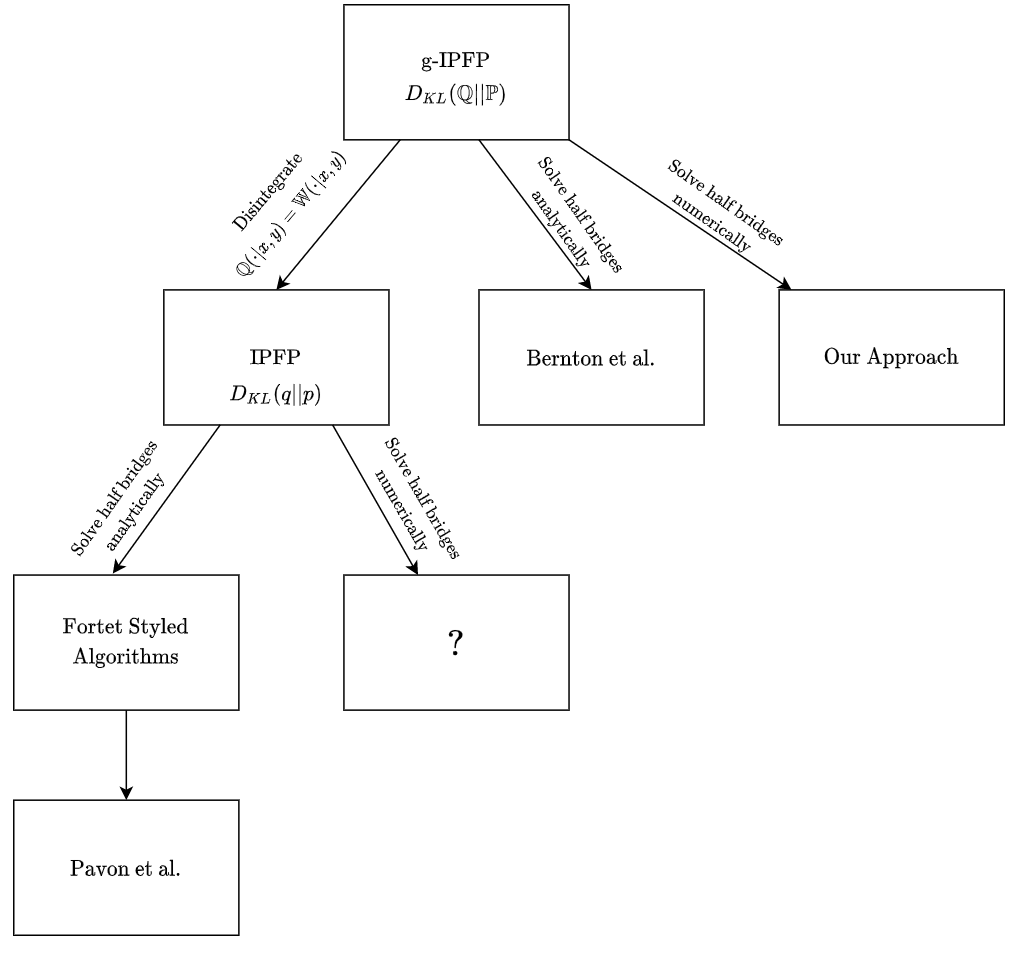
\includegraphics[width=\linewidth]{images/IPFP_Geanology.png}
    \caption{Genealogy of IPFP based algorithms for solving the Schrödinger. ? Symbolises an area open for development. Diagram could be more fine-grained in terms of the approach i.e. whether it is the control formulation of the problem. }
    \label{fig:genealogy}
\end{figure}

%\chapter{Related Work} 
\chapter{Related Problems}
\section{Continuous Time Stochastic Flows}

Imagine as probabilistic modeller you were given the problem of mapping from one distribution to another. One of the simplest ways of going about such task is to specify a generative process of the form:
\begin{align*}
    \rvx &\sim \pi_0 \\
    \rvy &= \calT_{\theta}(\rvx)
\end{align*}
Where $\calT_{\theta}(\rvx)$  is a stochastic mapping (i.e. $\calT_{\theta}(\rvx) = f_{\theta}(\rvx) + \rvepsilon$). Then we maximise the marginal likelihood for a set of observations $\{\vy_i \sim \pi_1 \}$:
\begin{align*}
    \prod_i p(\vy_i) = \prod_i \int p_{\theta}(\vy_i | \vx) d\pi_0(\vx)
\end{align*}

We can take a further step and model the relationship between the two distributions using an SDE:
\begin{align*}
    \rvx &\sim \pi_0 \\
    d\rvx(t) &= \vb_{\theta}(\rvx(t), t) + \gamma d\rvw(t) \\
    \rvy &= f_{\theta}(\rvx(1)),
\end{align*}
in other words $\rvy$ is generated by the solutions to an SDE with initial distribution $\pi_0$. We can also interpret the above as the latent object living in path space as we have no observations for the trajectories  but only observations of its initial and terminal distributions. Then similarly to the latent variable model example we aim to maximise an estimate of the marginal likelihood under this generative process. Variants of this approach are explored \citep{lahdesmakideep, tzen2019neural} as ways of having infinitely deep neural networks and Gaussian processes.

It is clear that this approach is different to the Schrödinger Bridge, first the generative process requires to observe pairs $\vx_i, \vy_i$ in order to estimate the marginal likelihood. Secondly the Schrödinger bridge is based on a principle of maximum entropy whilst this generative approach is based on maximum likelihood (ML-II).  However they share the similarity of exploiting stochastic dynamics to relate source and target distributions, both have similar notions of prior and posterior dynamics in them.

\section{Domain Adaptation and Generative Adversarial Networks (GANs)}

In this section we will motivate and provide some formal arguments towards the following observation:
\begin{observation}
Each half-bridge objective in the IPFP algorithm is equivalent to a GAN like objective with a corresponding cycle-consistency term up to a custom regularisation term.
\end{observation}

\subsection{Short Introduction to Domain Adaptation via GANs}

The goal of a GAN is to fit a generative model of the form:
\begin{align*}
    \rvx &\sim \pi_0 \\
    \rvy &= f_{\theta}(\rvx).
\end{align*}
In the setting where we can sample from $\pi_0(\vx)$ and $\pi_1(\vy)$ tractably. note that the above model induces likelihood $p_{\theta}(\vy | \vx)$ and marginal $p_{\theta}(\vy)$, however the marginal is never computed explicitly and thus sometimes fitting GANs is refered to as fitting implicit generative models \citep{mohamed2016learning}.

To recap what a the GAN fitting procedure \citep{goodfellow2014generative} looks like in our notation its the following two steps:

\begin{itemize}
    \item (Discriminator loss) Estimating the surrogate to later be fitted by model $p_{\theta}(y)$:
 $$ {\beta}^{*} = \argmin_{\phi} \alpha \E_{\pi_1(\vy)}[-\log D_{\beta}(\vy)] + (1-\alpha)\E_{p_{\theta}(\vy)}[-\log (1-D_{\phi}(\vy))]$$ 
 \item (Generative loss) Fitting model $p_{\theta}(\vy)$ on the estimated surrogate:
 $$\theta^{*} = \argmin_{\theta}-\E_{p_{\theta}(\vy)}\left[\log(D_{\hat{\phi}}(\vy))\right] $$ 
\end{itemize}

The generator step in practice for GANs \citep{goodfellow2014generative} typically minimises $-\E_{p_{\theta}(\vy)}\left[\log(D(\vy))\right]$  , following \cite{goodfellow2014generative} this is equivalent to maximising  $\E_{p_{\theta}(\vy)}\left[\log(1-D(\vy))\right]$.

The task of domain adaptation in GANs is that of finding mapping / alignment between two distributions $\pi_0, \pi_1$ that have been observed empirically. This has observations in image and language translation \citep{zhu2017unpaired,lample2017unsupervised}. Typically in domain adaptation with GANs the following two processes are fitted in parallel:
\begin{align*}
    \rvx &\sim \pi_0    &\rvy &\sim \pi_1\\
    \rvy &= f_{\theta}(\rvx)   &\rvx &= g_{\phi}(\rvy).
\end{align*}
An interesting variations of GANs used for domain adaptation known as cycle-GAN add an extra term to the generative loss coined the cycle-consistency loss:
\begin{align*}
   \E_{\vx \sim \pi_0}\left[ \Big|\Big|\vx- g_\phi\left(f_\theta(\vx) \right) \Big|\Big|^2\right] +  \E_{\vy \sim \pi_1}\left[ \Big|\Big|\vy- f_\theta\left(g_\phi(\vy) \right) \Big|\Big|^2\right]
\end{align*}
these auto-encoder losses ensure that the transformations learned from one data-set to another are inverses of each other. We will show in the next section how this cycle consistency term pops out naturally from the Schrödinger bridge problem.

\subsection{Connection To IPFP}
Starting from the static formulation of the problem
\begin{align*}
\argmin_{q(\vx,\vy) \in \mathcal{D}(\pi_0, \pi_1)}- \int q(\vx,\vy) \log p^{\W^{\gamma}}(\vx ,\vy )d\vx d\vy +\int q(\vx,\vy) \log q(\vx ,\vy )d\vx d\vy
\end{align*}
Now let us consider the backwards step in IPFP for the $i$-th iteration:
\begin{align*}
\arginf_{p(\vx,\vy)  \in \mathcal{D}(\pi_1)}- \int p(\vx,\vy)  \log q^{i-1}(\vx,\vy)d\vx d\vy +\int  p(\vx,\vy) \log  p(\vx,\vy) d\vx d\vy
\end{align*}
we can enforce this constraint using the product rule i.e. $p(\vx,\vy) = p_{\phi}(\vx|\vy) \pi_1(\vy)$ (we can parametrise $p_{\phi}(\vx|\vy)$ with a powerful estimator):
\begin{align*}
\argmin_{\phi}&\!\!-\!\!\int\!\!p_{\phi}(\vx|\vy) \pi_1(\vy) \log q^{i-1}(\vx,\vy)d\vx d\vy\!+\!\!\!\int\!\!p_{\phi}(\vx|\vy) \pi_1(\vy) \log p_{\phi}(\vx|\vy)
\pi_1(y)d\vx d\vy\\
\argmin_{\phi}&- \int p_{\phi}(\vx|\vy) \pi_1(\vy) \log q^{i-1}(\vx,\vy)d\vx d\vy +\int p_{\phi}(\vx|\vy)\pi_1(\vy) \log q_{\phi}(\vx|\vy)
d\vx d\vy
\end{align*}
Now following our selected parametrisation if we are beyond the first iteration the product rule yields $q^{i-1}(\vx , \vy)= q^{i-1}_{\theta}(\vy|\vx)\pi_0(\vx)$
\begin{align*}
\argmin_\theta&- \int p_{\phi}(\vx|\vy) \pi_1(\vy) \log  q^{i-1}_{\theta}(\vx|\vy)dxdy - \int p_{\phi}(\vx|\vy) \pi_1(\vy) \log  \pi_0(\vx) d\vx d\vy \\
&+\int p_{\phi}(\vx|\vx) \pi_1(\vy) \log p_{\phi]}(\vx|\vy)d\vx d\vy 
\end{align*}
Simplifying further:
\begin{align*}
\argmin_\phi- \E_{p_{\phi}(\vx|\vy)\pi_1(\vy)}\left[  \log  q^{i-1}_{\theta}(\vy|\vx)\right] -  \E_{p_{\phi}(\vx)}\left[ \log  \pi_0(\vx) \right] - H\left(p_{\phi}(\vx|\vy)\pi_1(\vy)\right)
\end{align*}

Sampling from $p_{\phi}(\vy|\vx)\pi_1(y)$ can be achieved via  ancestral sampling and we can parametrise $p_{\phi}(\vy|\vx)=\calN(\vx | \mu_{\phi}(\vy), \sigma^2_\phi(\vy))$ following \cite{kingma2013auto} such that it is easy to sample conditioned on $\vy$. Under the discussed parametrisations expectations are taken with respect to the empirical distribution via ancestral sampling and thus we don't require any importance sampling or the likes, however we have introduced some bias by parametrising $p_{\phi}(\vy|\vx)$ with a class of distributions.

What is more interesting is that the above objectives is very similar to the cycle-GAN \citep{zhu2017unpaired} objective which gives us a nice link to a wide variety of successful empirical methods:

Backwards step:
\begin{align*}
\argmin_\phi- \E_{p_{\phi}(\vy|\vx)\pi_1(\vy)}\left[  \log  q^{i-1}_{\theta}(\vy|\vx)\right] -  \E_{p_{\phi}(\vx)}\left[ \log  \pi_0(\vx) \right] - H\left(p_{\phi}(\vy|\vx)\pi_1(\vy)\right)
\end{align*}
Forwards step:
\begin{align*}
\argmin_\theta- \E_{q_{\theta}(\vy|\vx)\pi_0(\vx)}\left[  \log  p^i_{\phi}(\vy|\vx)\right] -  \E_{q_{\theta}(\vy)}\left[ \log  \pi_1(\vy) \right] - H\left(q_{\theta}(\vy|\vx)\pi_0(\vx)\right)
\end{align*}

\begin{observation}\label{obs:cycle}
Using our proposed parametrisation we can see that the term:
$$\E_{q^i_{\theta}(\vy|\vx)\pi_0(\vx)}\left[  \log  p^i_{\phi}(\vy|\vx)\right] \propto \E_{\pi_0(\vx)\calN(\epsilon|\textbf{0},\I )}\left[  -  \frac{1}{2\sigma_x^2}\Big|\Big|\vx- \mu_\phi\left(\mu_\theta(\vx) + \sigma_y \bm{\epsilon}\right) \Big|\Big|^2\right],$$
matches the corresponding the cycle-consistency loss terms in cycle GAN \cite{zhu2017unpaired} in the $\sigma_y \downarrow 0$ limit.
\end{observation}
\begin{proof}

For simplicity lets make the variance function independent of the input $\sigma^2_{\theta}(\vx) = \sigma_{x}^2 \I$ 
\begin{align*}
\E_{q_{\theta}(\vy|\vx)\pi_0(\vx)}\left[  \log  p^i_{\phi}{\phi}(\vy|\vx)\right] \propto \E_{q_{\theta}(\vy|\vx)\pi_0(\vx)}\left[  -  \frac{1}{2\sigma_x^2}||\vx- {\mu}_{\phi}(\vy))||^2\right]
\end{align*}
We can apply the reparametrisation trick \cite{kingma2013auto} to $p_{\theta}(\vy|\vx)\pi_0(\vx)$ : 
\begin{align*}
    \vx &\sim \pi_0(\vx) \\
    \vy &= {\mu}_{\theta}(\vx) + \sigma_y \bm{\epsilon} \quad \bm{\epsilon} \sim \calN(\textbf{0}, \I)
\end{align*}

Using the above reparametrisation we can re-write the cross-term loss as : 

\begin{align*}
 \E_{q_{\theta}(\vy|\vx)\pi_0(\vx)}\left[  \log  p^i_{\phi}{\phi}(\vy|\vx)\right] \propto \E_{\pi_0(\vx)\calN(\epsilon|\textbf{0},\I )}\left[  -  \frac{1}{2\sigma_x^2}\Big|\Big|\vx- \mu_\phi\left(\mu_\theta(\vx) + \sigma_y \bm{\epsilon}\right) \Big|\Big|^2\right]
\end{align*}

Where $ -  \frac{1}{2\sigma_x^2}\Big|\Big|\vx- \mu_\phi\left(\mu_\theta(\vx) + \sigma_y \bm{\epsilon}\right) \Big|\Big|^22$ takes the same autoencoder(AE) form as the cycle consistency loss in cycle GAN with some added noise (they are related asymptotically in the zero noise limit just like VAEs and AEs).
\end{proof}

For notational simplicity we have treated the the $\sigma_i$ terms as constants in the above derivations, adapting the above argument to their non-constant counterparts is simple and does not add much to Observation \ref{obs:cycle}.


 Now we will focus on the connection between our remaining terms and the generative loss:

\begin{observation}
Up to optimisation constants and for the optimal discriminator $D^{*}$ and a generator $q_{\theta}(\vy | \vx)$ as defined in \citep{goodfellow2014generative,mohamed2016learning}, we have the following:
\begin{align*}
-\E_{q_{\theta}(\vy)}\left[ \log  \pi_1(\vy) \right] \propto-\E_{q_{\theta}(\vy)}\left[\log(D^{*}(\vy))\right] - \E_{q_{\theta}(\vy)}\left[\log\left(q_{\theta}(\vy) + \pi_1(\vy)\right)\right],
\end{align*}
In short we can express cross entropy between our model and the empirical distribution in terms of of the optimal discriminator $D^{*}$ and a further term (which is one of the terms in the Jensen Shannon Divergence - JSD ). 
\end{observation}
\begin{proof}

Using the ratio expression from \cite{mohamed2016learning}
\begin{align*}
\log D^{*}(\vy) &= \log\left(\frac{\pi_1(\vy)p(c=1)}{p(\vy)}\right) \\
&=\log\left(\frac{\pi_1(\vy)p(c=1)}{p(c=1)p(y|c=1) + p(c=0)p(\vy|c=0)}\right) \\
&= \log\left(\frac{\pi_1(\vy)\alpha}{\alpha\pi_1(\vy) + (1-\alpha)  p_{\theta}(\vy)}\right) \\
&\propto \log\left(\pi_1(\vy)\right) - \log\left(\alpha\pi_1(\vy)  + (1-\alpha)p_{\theta}(\vy) \right)
\end{align*}

Considering the case for $\alpha=\frac{1}{2}$ we have : 
\begin{align*}
\log D^{*}(\vy) \propto \log\left(\pi_1(\vy)\right) - \log\left(q_{\theta}(\vy) + \pi_1(\vy)\right)
\end{align*}

thus:
\begin{align}\label{eq:gan_entropy}
\E_{q_{\theta}(\vy)}\left[\log D^{*}(\vy)\right] \propto \E_{q_{\theta}(\vy)}\left[\log\left(\pi_1(\vy)\right)\right] -\E_{q_{\theta}(\vy)}\left[\log\left(q_{\theta}(\vy) + \pi_1(\vy)\right)\right]
\end{align}

\end{proof}

The above observation hold true for an optimal classifier $D^{*}$ that can tell apart samples from $\pi_\theta(\vy)$ and $\pi_1(\vy)$ see \cite{mohamed2016learning} for furhter motivations. The main differences we have in each half bridge objective is the additional entropy term which helps with making our estimates spread out, whilst GANs instead have one of the terms from the JSD.  So up to a term IPFP has two GANs trained until convergence going forwards and backwards in turn.

Lets quickly zoom into the terms that differ between our loss and the GAN loss removing constants the terms are:

\begin{align}
 \E_{q_{\theta}(\vy|\vx)\pi_0(\vx)}\left[ \log q_{\theta}(\vy|\vx) \right]\quad &\text{vs} \quad  \E_{q_{\theta}(\vy)}\left[\log\left(q_{\theta}(\vy) + \pi_1(\vy)\right)\right]
\end{align}

The term $H_{\theta}(\vy|\vx) =\E_{q_{\theta}(\vy|\vx)\pi_0(\vx)}\left[ \log q_{\theta}(y|x) \right]$ is a conditoinal entropy whilst the term $\E_{q_{\theta}(\vy)}\left[\log\left(q_{\theta}(\vy) + \pi_1(\vy)\right)\right]$ is one of the terms in the Jensen Shanon divergence, both prevent the delta collapse of the reverse cross entropy, and is the main difference between GANs and a single forward (or backwards) pass of IPF on the schrodinger bridge problem.

 Note than under this parametrisation the term $H_{\theta}(\vy|\vx)$ can be obtained in closed form $\E_{\pi_1(\vy)}[\log {\sigma}_{\theta}(\vy)]$ and has the clear interpretation in that it maximises the variance / spread of our mapping.
 
 The above results raise an interesting question: Is it possible to train GANs for domain adaptation by alternating  half bridge styled GAN iterations until convergence as some form of approximate IPFP? the additional term difference from the half bridges removes the theoretical support from this proposed heuristic nonetheless there might still be a further relationship that we may have missed between the two such as a lower bound.



%\chapter{Design and Implementation}
\chapter{Empirical Schrödinger Bridges}

Now we have finally reached the core section of this thesis, were we propose and discuss numerical implementations for the Schrodinger Bridge Problem. We call the Empirical Schrodinger Bridge, the setting of the Schrodinger bridge problem when the marginal/boundary distributions are only available via samples (i.e. their empirical distribution):
\begin{align}
    \hat{\pi}_0(\vx)  = \frac{1}{N}\sum_i \delta(\vx -\vx_i) &, \quad\hat{\pi}_1(\vy)  = \frac{1}{M}\sum_j \delta(\vy -\vy_j) \nonumber\\
    \vx_i \sim \pi_0 &, \quad \vy_j \sim \pi_1
\end{align}

Note that \cite{pavon2018data} refer to this problem as the Data Driven Schrodinger Bridge. We will discuss  different algorithms derived from the g-IPFP for solving the Schrodinger Bridge under this Empirical setting. As this is a fairly new problem of interest in the applied/numerical setting there is not much accessible and validated prior work out there already thus for prior approaches will will only be reproducing and commenting on the work of \cite{pavon2018data}.

Our main contributions are:

\begin{itemize}
    \item The proposal of two completely new numerical algorithms for solving the empirical Schrodinger bridge problem.
    \item The rephrasing of the Method by \cite{pavon2018data} as an un-normalised likelihood estimation problem and connection to alternative methods within the Machine Learning and applied statistics community.
\end{itemize}

\section{Direct Half Bridge Drift Estimation with Gaussian Processes}

In this approach we wish to exploit the fact that we have an expression for the path measure that globally solves for the half bridge problems.  Thus rather than parametrise the optimisation problem in the half bridge and solve that numerically, here we seek to directly approximate the measure that solves for the half bridge via a Gaussian process estimate of the drift on trajectories sampled from the optimal measure.

We start from the following observation which in short tells us how to sample from the optimal distribution that solves the half bridge:
\begin{observation}
Given that we can parametrise a measure $\W$ with its drift as the weak solution to the following SDE:
\begin{align*}
    d\rvx^{\pm}(t) =  \pm \rvb^{\pm}(t) + \gamma d \rvw^{\pm}(t) 
\end{align*}
Then we can sample from the solution to the following half bridges:
\begin{align*}
   \P^{*-} = \arginf_{\P \in \calD(\cdot,\pi_1)}\KL(\P || \W) \\ 
   \P^{*+} = \arginf_{\P \in \calD(\pi_0,\cdot )}\KL(\P || \W)
\end{align*}
via simulating trajectories (i.e. via EM) using the following SDEs respectively:
\begin{align*}
     d\rvx^{-}(t) &=  - \rvb^{-}(t) + \gamma d \rvw^{-}(t) , \quad  \rvx(1) \sim \pi_1, \\
     d\rvx^{+}(t) &=  \rvb^{+}(t) + \gamma d \rvw^{+}(t) , \quad  \rvx(0) \sim \pi_0.
\end{align*}
That is paths sampled from the above SDEs will be distributed according to $\P^{*-}$ and $\P^{*+}$ respectively.
\end{observation}
\begin{proof}(Sketch.) This is nothing but enforcing the constraints via the product rule (disintegration theorem) and then matching the remainder of the unconstrained interval with the prior distribution $\W$ following Theorems \ref{thrm:half_bridge_forward}, \ref{thrm:half_bridge_backward}.
\end{proof}
Intuitively we are performing a surgery styled operation by cutting and pasting over the dynamics on the shortened (unconstrained) time interval and attaching the constraint to it at the corresponding boundary.
\begin{figure}
    \centering
    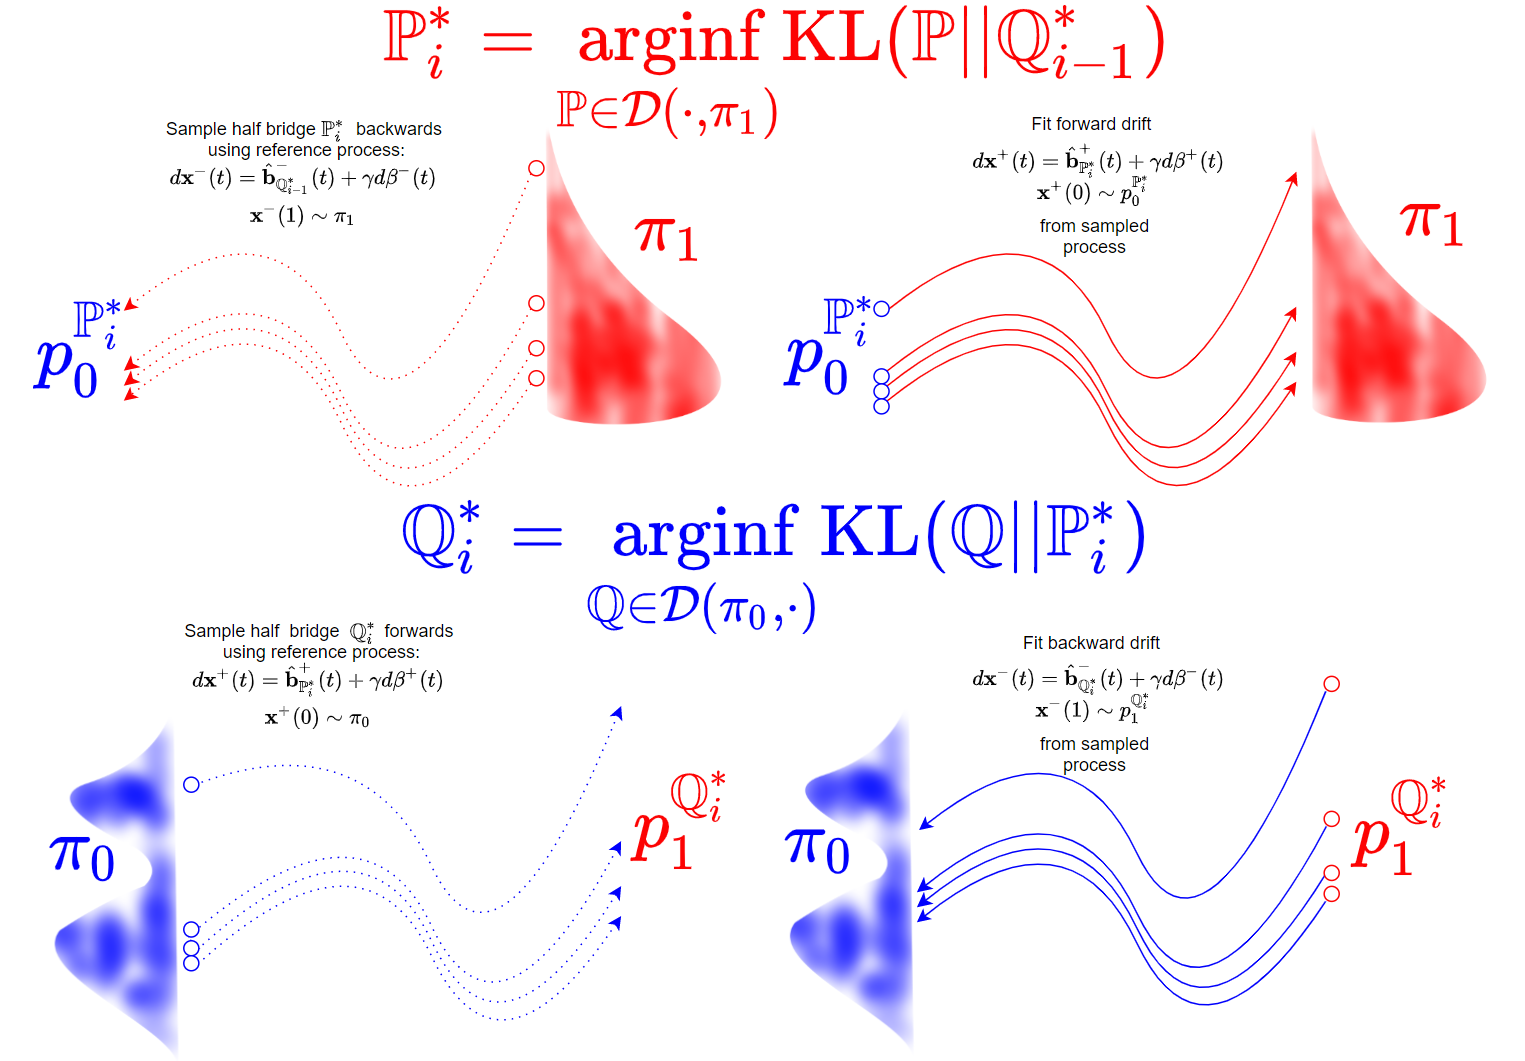
\includegraphics[width=\linewidth]{images/gp_IPFP.PNG}
    \caption{$i^{\text{th}}$ Iteration for drift based approximation to g-IPFP. In each iteration we draw samples from the process in the direction that incorporates the constraint as an initial value, and we learn the drift which simulates the same path measure in the opposite direction to the sampling. With each iteration $\mathbf{\color{blue}{p^{\P^{*}_i}_0}}$ and $\mathbf{\color{red}{p^{\Q^{*}_i}_1}}$ get close to $\mathbf{\color{blue}{\pi_0}}$ and $\mathbf{\color{red}{\pi_1}}$ respectively}
    \label{fig:gp_drift}
\end{figure}
\subsection{Fitting the Drift from Samples}

Once we have sampled trajectories from the half bridge solution ($\{\vx^{+}_i(t_k)\}_{i,k}^N$ or  $\{\vx^{-}_j(t_l)\}_{j,l}^M$ ) we  apply the methodology from \cite{ruttor2013approximate} in order to infer the drift:

Via the Euler-Mayurama discretisations we have that the transition probabilites follow a Gaussian distribution:

For the backwards samples, we wish to infer the forwards drift:
\begin{align*}
    p&\left(\{\vx^{-}_j(t_l)\}_{l}^M \Big| \vb^{+}_{\P_{i}}(\cdot, \cdot)\right) \propto\\
    &\prod \exp \left( -\frac{1}{2\Delta t} ||\vx^{-}_j(t_l) - \vx^{-}_j(t_l - \Delta t) -  \Delta t\vb^{+}_{\P_{i}}\left(\vx^{-}_j(t_l - \Delta t), t_l - \Delta t\right) ||^2 \right), 
\end{align*}
and conversely for forwards samples, we wish to infer the backwards drift:
\begin{align*}
    p&\left(\{\vx^{-}_j(t_l)\}_{l}^M \Big| \vb^{-}_{\Q_{i}}(\cdot, \cdot)\right) \propto\\
    &\prod \exp \left( -\frac{1}{2\Delta t} ||\vx^{-}_j(t_l - \Delta t)  - \vx^{-}_j(t_l)  +  \Delta t\vb^{-}_{\Q_{i}}\left(\vx^{-}_j(t_l - \Delta t), t_l - \Delta t\right) ||^2 \right), 
\end{align*}
placing Gaussian process priors on the drift functions $\vb^{-}_{\Q_{i}}$ and $\vb^{+}_{\P_{i}}$ we arrive at the following multioutput GP regression problems:
\begin{align*}
        \frac{\vx^{-}_j(t_l) - \vx^{-}_j(t_l - \Delta t)}{\Delta t} = \vb^{+}_{\P_{i}}\left(\vx^{-}_j(t_l - \Delta t), t_l - \Delta t\right) +\frac{\bm{\sigma}}{\Delta t}\epsilon ,\\
        \frac{\vx^{-}_j(t_l - \Delta t)  - \vx^{-}_j(t_l)}{\Delta t}  = -\vb^{-}_{\Q_{i}}\left(\vx^{-}_j(t_l - \Delta t), t_l - \Delta t\right) +\frac{\bm{\sigma}}{\Delta t}\epsilon,
\end{align*}
where
\begin{align}
   \vb^{+}_{\P_{i}} \sim \mathcal{GP} \quad \vb^{-}_{\Q_{i}} \sim \mathcal{GP}\quad \epsilon \sim \calN(\vzero, \I).
\end{align}
Following \cite{ruttor2013approximate} we assume the dimensions of the drift function are independent (which is equivalent to imposing a block diagonal kernel matrix on a multi-output GP) and thus we fit a separate GP for each dimension, yielding the following predictive mean per dimension $k$ of the drift:
\begin{align}
[\bar{\vb}^{+}_{\P_{i}}(\vx, t)]_k = \vk_k^{+}(\vx \oplus t)^{\top} \left(\mK_k^{+} + \frac{(\sigma_k^{+})^2}{\Delta t} \I\right)^{-1}\!\!\!\!\!\!\vy_k^{+}, \\
[\vb^{-}_{\Q_{i}}(\vx, t)]_k = \vk_k^{-}(\vx \oplus t)^{\top} \left(\mK_k^{-} + \frac{(\sigma_k^{-})^2}{\Delta t} \I\right)^{-1}\!\!\!\!\!\!\vy_k^{-} ,
\end{align}
where:
\begin{align*}
   &[ \mK_k^{+} ]_{il} = {K}\big([\vx^{-}_j(t_i- \Delta t)]_k\oplus t_i - \Delta t, [\vx^{-}_j(t_i - \Delta t)]_k \oplus t_l - \Delta t \big) \\
   &[ \mK_k^{+} ]_{il} = {K}\big([\vx^{+}_j(t_i)]_k \oplus t_i , [\vx^{+}_j(t_i)]_k\oplus t_l \big)  \\
   &\vy_k^{+} =  \left[\frac{\vx^{-}_j(t_l) - \vx^{-}_j(t_l - \Delta t)}{\Delta t}\right]_k \quad \vy_k^{-} =  \left[\frac{\vx^{-}_j(t_l - \Delta t)  - \vx^{-}_j(t_l)}{\Delta t} \right]_k
\end{align*}
In practice we are not making use of the predictive variances \footnote{we are effectively just doing Kernel Ridge Regression.}. Instead we just use the predictive mean as an estimate for the drift and subsequently use that estimate to run the EM method required in this flavour of approximate g-IPFP.


Now we have the relevant ingredients to carry out this flavour of approximate g-IPFP specified in Algorithm  \ref{alg:gp_gipfp}.
%  $\{\vx^{+}_i(t_k)\}_{i,k}^N$ or  $\{\vx^{-}_j(t_l)\}_{j,l}^M$
\begin{algorithm} \label{alg:gp_gipfp}
\SetKwInOut{Input}{input}
\Input{$\pi_0(\vx), \pi_1(\vy), \W^{\gamma}$}
Initialise:\\
$i=0$ \\
$\Q^{*}_0 =\W^{\gamma}$\\
Obtain or estimate backwards drift of prior: \\
$\bar{\vb}^{-}_{\Q_{0}}(\vx, t) := \text{ObtainBackwardDrift}(\Q^{*}_0)$\\

\Repeat{convergence}{
      $i := i + 1$ \\
      $\{\vx^{-}_j(t_l)\}_{j,l}^M = \text{SDESolve}\Big(-\bar{\vb}^{-}_{\Q_{i-1}}, \gamma, \pi_1, \Delta t, M\Big)$\\
     $ \bar{\vb}^{+}_{\P_{i}} := \text{GaussianProcessDriftEstimate}\Big( \{\vx^{-}_j(t_l)\}_{j,l}^M, \, \text{forwards=True} \Big)$\\ 
     $\{\vx^{+}_n(t_k)\}_{n,k}^N = \text{SDESolve}\Big(\bar{\vb}^{+}_{\P_{i}}, \gamma, \pi_0, \Delta t, N\Big)$ \\
     $\bar{\vb}^{-}_{\Q_{i}} := \text{GaussianProcessDriftEstimate}\Big( \{\vx^{+}_n(t_k)\}_{n,k}^N, \, \text{forwards=False} \Big)$
    }
\Return{$\bar{\vb}^{-}_{\Q_{i}}, \bar{\vb}^{+}_{\P_{i}}$}
\caption{ Approximate g-IPFP with Gaussian processes   }
\end{algorithm}

Where the $\text{SDESolve}\Big(-\bar{\vb}^{-}_{\Q_{i-1}}, \gamma, \pi_1, \Delta t, M\Big)$ routine generates $M$ trajectories using the Euler-Mayurama method.

\subsubsection{Sampling a Reverse-time Difussion }
A quick note to the reader is that the sign multiplying the drift in line $8$ of Algorithm \ref{alg:gp_gipfp} may seem a bit ad-hoc however we can motivate it via seeing Ito-process as the continuous time limit of discrete time Markov chains:

We want to consider the case where both backwards and forward transitions  obey the same joint probability law, that is:
\begin{align}\label{eq:markov_e}
    p^{+}(\vx_{t+\Delta t}|\vx_t)p_t(\vx_t)=p^{-}(\vx_t|\vx_{t+\Delta t})p_{t+\epsilon}(\vx_{t+\Delta t}),
\end{align}
where $p_t(\cdot)$ is the marginal distribution at time $t$. $p^{+}(\cdot|\cdot)$ and $p^{-}(\cdot|\cdot)$ are Gaussian's of the form:
\begin{align*}
p^{+}(\vx_{t+\Delta t}|\vx_t)&=\frac{1}{2\pi \Delta t }\exp\left(-\frac{1}{2\Delta t}\left[\vx_{t+\Delta t}-(\vx_t+\vb^{+}(\vx_t,t)\Delta t)\right]^2\right) \\
p^{-}(\vx_t|\vx_{t+\Delta t})&=\frac{1}{2\pi \Delta t}\exp\left(-\frac{1}{2\Delta t}\left[\vx_t-\left(\vx_{t+\Delta t}-\vb^{-}(\vx_{t+\Delta t},t+\Delta t)\Delta t\right)\right]^2\right).
\end{align*}
Taking logs on Equation \ref{eq:markov_e} and preserving a linear order in $\Delta t$ gives
\begin{align*}
    (\vb^+(\vx_t,t)-\vb^-(\vx_{t+\Delta t},t+\Delta t)(\vx_{t+\Delta t}-\vx_t)=\log p_{t+\Delta t}(\vx_{t+\Delta t}) - \log p_t(\vx_t), 
\end{align*}
which in the continuous time limit arrives to our chosen flavour \footnote{Different authors parametrise the duality formula with different signs in result changing the sign of the EM discretisation.} of Nelson's duality formula:
\begin{align*}
      \vb^+(\vx_t,t) -\vb^-(\vx_t,t) = \nabla\log p(\vx_t, t)
\end{align*}

\section{Stochastic Control Approach}

We would like to carry out a variant of g-IPFP that is based on the stochastic control formulations of the half bridge problems. Via a slight adaptation of Lemma \ref{lemma:control} we can re-write the half bridge steps of g-IPFP as:
\begin{itemize}
\item Backward Half bridge (time-reversed dynamics): 
\begin{align} \label{eq:controlled_haalf_bridge_forward}
  \rvb^{-}_{\P_{i}}(t) = \min_{\rvb^{-} \in \calB }  &\E_\P\left[\int_0^1 \frac{1}{2\gamma}\big|\big|\rvb^{-}(t) -\rvb^{-}_{\Q_{i-1}}(t) \big|\big|^2 dt\right] \nonumber \\
    s.t.\;\;\; d\rvx(t) = \rvb^{-}(t) &dt + \sqrt{\gamma} \rvw^{-}(t), \;\; \rvx(1) \sim \pi_1
\end{align}
\item Forward Half bridge:
\begin{align} \label{eq:controlled_half_bridge_backward}
   \rvb^{+}_{\Q_{i}}(t) =\min_{\rvb^{-} \in \calB } & \E_\Q\left[\int_0^1 \frac{1}{2\gamma}\big|\big|\rvb^{+}(t) -\rvb^{+}_{\P_{i}}(t)\big|\big|^2 dt\right] \nonumber \\
    s.t.\;\;\; d\rvx(t) = \rvb^{+}(t) &dt + \sqrt{\gamma} \rvw^{+}(t), \;\; \rvx(0) \sim \pi_0
\end{align}.
\end{itemize}
Where the dual drifts can be obtained via Nelson's duality equation:
\begin{align*}
      \rvb^{-}_{\Q_{i-1}}(t)   &=\rvb^{+}_{\Q_{i-1}}(t) -\gamma\nabla_{\vx} p^{\Q_{i-1}}(\rvx(t), t) \\
    \rvb^{+}_{\P_{i}}(t) &=  \rvb^{-}_{\P_{i}}(t) +\gamma\nabla_{\vx} p^{\P_{i}}(\rvx(t), t)
\end{align*}
Note that we carry express the dynamical evolution for $\P$ in the backwards half bridge as a time reversed process \citep{pavon1991free, nelson1967dynamical} such that the terminal distribution constraint $\rvx(1) \sim \pi_1$ becomes an initial value problem in reversed time, which is something we know how to sample from. 

Now in theory we have all the elements to carry out g-IPFP under this control formulation, however note that the dual drifts require the gradient of the solution to their respective Fokker-Plank equations (i.e. $\nabla_{\vx} p^{\P_{i}}(\rvx(t), t)$, $\nabla_{\vx} p^{\Q_{i-1}}(\rvx(t), t)$). Estimating $p^{\P_{i}}(\rvx(t), t)$ or $p^{\Q_{i-1}}(\rvx(t), t)$ is going to be very costly since we  will also need to evaluate such estimations for every point in the interval $[0,1]$ that we use to estimate the integral $\int_0^1 \hdots dt$.

\subsection{Forwards and Backwards Diffusion's}

As mentioned earlier Equations \ref{eq:controlled_half_bridge_backward}, and \ref{eq:controlled_haalf_bridge_forward} exhibit the computational challenge of estimating solutions to the FPK equation along trajectories in $[0,1]$.  In order to overcome this we will derive alternate expressions for Equations \ref{eq:controlled_half_bridge_backward},  \ref{eq:controlled_haalf_bridge_forward} that do not involve FPK solution terms inside the time integral (path functional).
\begin{proposition}\label{prop:halfforcontrol}
The Forward half bridge (We set $\gamma=1$  for simplicity):
\begin{align*} 
   \rvb^{+}_{\Q_{i}}(t) =\min_{\rvb_\Q^{-} \in \calB } & \E_\Q\left[\int_0^1 \frac{1}{2}\big|\big|\rvb_\Q^{+}(t) +\rvb^{+}_{\P_{i}}(t)\big|\big|^2 dt\right] \nonumber \\
    s.t.\;\;\; d\rvx(t) = \rvb_\Q^{+}(t) &dt +  \rvw^{+}(t), \;\; \rvx(0) \sim \pi_0
\end{align*}
can be expressed as:
\begin{align} \label{eq:div_control_forward}
   \rvb^{+}_{\Q_{i}}(t) =\min_{\rvb^{-} \in \calB } -2\E_{p^{\Q}_1}\left[\log \pi_1 \right] &+ \E_{\Q}\left[\int_0^1 \left(\frac{1}{2}(b_\Q^{+}(t) - b_{\P_{i}}^{-}(t))^2 - \nabla\cdot b^{-}_{\P_{i}}(t) \right)\right] \nonumber \\
    s.t.\;\;\; d\rvx(t) = \rvb_\Q^{+}(t) &dt + \rvw^{+}(t), \;\; \rvx(0) \sim \pi_0
\end{align}.
\end{proposition}
\begin{proof}
First lets  abbreviate  terms of the form $p^{\X}(\rvx(t), t)$ with $p^{\X}_t$ and $b^{\X}_{\pm}(t)$ with $b^{\X}_{\pm}$ for compactness purposes. Lets express the KL in terms of backwards drifts (known result):
\begin{align}
\KL(\Q||{\P_{i}}) = \KL( p_0^{\Q}|| p_0^{{\P_{i}}}) + \frac{1}{2}\E_{\Q}\left[\int_0^1 ( b_\Q^{+} - b^{\P_{i}}_{+})^2 dt\right].
\end{align}
Using Nelson's duality formula $b^{\P_{i}}_+(t) =b^{\P_{i}}_-(t) + \nabla\log p_t$:
\begin{align}
\KL(\Q||{\P_{i}}) = \KL( p_0^{\Q}|| p_0^{{\P_{i}}}) + \frac{1}{2}\E_{\Q}\left[\int_0^1 ( b_\Q^{+} - b_{\P_{i}}^{-} - \nabla\log p_t^{\P_{i}})^2 dt\right].
\end{align}
Expanding:
\begin{align*}
\KL(\Q&||{\P_{i}}) = \KL( p_0^{\Q}|| p_0^{{\P_{i}}}) +\\ &\frac{1}{2}\E_{\Q}\left[\int_0^1 \left(( b_\Q^{+} - b_{\P_{i}}^{-})^2 - 2\nabla\log p_t^{\P_{i}} \cdot ( b_\Q^{+} - b_{\P_{i}}^{-}) + {\nabla\log p_t^{\P_{i}}}^2 \right)dt\right].
\end{align*}
Using the chain rule for the second derivative $\Delta \log  p = -\frac{(\nabla p)^2}{ p^2}  + \frac{\Delta  p}{ p}$:
\begin{align*}
&\KL(\Q||{\P_{i}}) =\KL( p_0^{\Q}|| p_0^{{\P_{i}}}) +\\ &\frac{1}{2}\E_{\Q}\left[\int_0^1 \left(\!\!( b_\Q^{+} - b_{\P_{i}}^{-})^2 \!\!- 2\nabla\log p_t^{\P_{i}}\!\!\!\cdot \!( b_\Q^{+} - b_{\P_{i}}^{-}) - \Delta \log  p^{\P_{i}}\!\!\!+ \frac{\nabla  p^{\P_{i}}}{ p^{\P_{i}}}\!\!\right)dt\right].
\end{align*}

Using Ito's rule we can show the following is true: 
\begin{align*}
\E_\Q\left[\log p^{\P_{i}}_1-\log p^{\P_{i}}_0\right] = \E_\Q\left[\int dt \left(b_+^\Q\cdot\nabla\log p_t^{\P_{i}} + \frac{1}{2}\Delta \log p_t^{\P_{i}}\right)\right]\\
\E_\Q\left[\int dt \left(b_+^\Q\cdot\nabla\log p_t^{\P_{i}} \right)\right] = \E_\Q\left[\log p^{\P_{i}}_1-\log p^{\P_{i}}_0 - \int dt \left( \frac{1}{2}\Delta \log p_t^{\P_{i}}\right)\right]
\end{align*}

Quick proof sketch of the above step. Via Ito's formula we have:
\begin{align*}
d\log  p_t^{{\P_{i}}} = b_+^\Q\cdot\nabla\log p_t^{\P_{i}} dt + \frac{1}{2}\Delta \log p_t^{\P_{i}} dt + \nabla \log p_t^{\P_{i}} \cdot dW
\end{align*}
Which implies (via taking expectations on both sides wrt $\Q$ and then dividing by $dt$)
\begin{align*}
\partial_t \E_{\Q}[\log  p_t^{{\P_{i}}}] = \E_{\Q}{\left[b_+^\Q\cdot\nabla\log p_t^{\P_{i}} + \frac{1}{2}\Delta \log p_t^{\P_{i}}\right]}
\end{align*}
Then integrating both sides from $0$ to $1$ (and applying Fubbini) gives exactly the above result

Pluging this back into the KL (the laplacians cancel out):
\begin{align*}
\KL(\Q||{\P_{i}}) = &\E_\Q\left[-\log \frac{ p^{\P_{i}}_1}{ p^\Q_0}\right] \\+ &\frac{1}{2}\E_{\Q}\left[\int_0^1 \left(( b_\Q^{+} - b_{\P_{i}}^{-})^2 + 2\nabla\log p_t^{\P_{i}} \cdot b_{\P_{i}}^{-}+ \frac{\Delta  p^{\P_{i}}}{ p^{\P_{i}}}\right)dt\right].
\end{align*}
Now we use the fact that $ p_t^{\P_{i}}$ obeys the Fokker—Planck equation (this is the case for diagonal covariance Ito-Processes, otherwise we would have cross terms form the Hessian) see Equation 13.4 in \cite{nelson1967dynamical}\footnote{more generally we have $\pm\partial_t p_t^{\P_{i}} = \frac{1}{2}\Delta p_t^{\P_{i}}\mp\nabla\cdot(b_\pm^{\P_{i}} p_t^{\P_{i}})$}: 
\begin{align*}
-\partial_t p_t^{\P_{i}} = \frac{1}{2}\Delta p_t^{\P_{i}}+\nabla\cdot(b_{-}^{\P_{i}} p_t^{\P_{i}})
\end{align*}
Using the product rule : 
\begin{align*}
-\partial_t p_t^{\P_{i}} = \frac{1}{2}\Delta p_t^{\P_{i}}+  p_t^{\P_{i}} \nabla\cdot(b_{-}^{\P_{i}}) + b_{-}^{\P_{i}} \cdot \nabla p_t^{\P_{i}} \\
-\partial_t p_t^{\P_{i}} -  p_t^{\P_{i}} \nabla\cdot b_{-}^{\P_{i}}  = \frac{1}{2}\Delta p_t^{\P_{i}}+ b_{-}^{\P_{i}} \cdot\nabla  p_t^{\P_{i}}
\end{align*}
Dividing both sides by $ p_t^{\P_{i}}$:
\begin{align*}
-\partial_t \log  p_t^{\P_{i}} - \nabla\cdot b_{-}^{\P_{i}}  = \frac{1}{2}\frac{\Delta  p_t^{\P_{i}}}{ p_t^{\P_{i}}}+  b_{-}^{\P_{i}} \cdot \nabla \log  p_t^{\P_{i}}
\end{align*}
Pluging back into the KL we have:
\begin{align*}
\KL(\Q||{\P_{i}}) &= \E_\Q\left[-\log \frac{{ p^{\P_{i}}_1}^2}{ p^\Q_0  p_0^{{\P_{i}}}}\right] + \frac{1}{2}\E_{\Q}\left[\int_0^1 \left(( b_\Q^{+} - b_{\P_{i}}^{-})^2 - 2\nabla\cdot b_{-}^{\P_{i}} \right)dt\right]. \\
D(\Q||{\P_{i}}) &= \E_\Q\left[-\log \frac{{ p^{\P_{i}}_1}^2}{ p^\Q_0   p_0^{{\P_{i}}}}\right] + \E_{\Q}\left[\int_0^1 \left(\frac{1}{2}( b_\Q^{+} - b_{\P_{i}}^{-})^2 - \nabla\cdot b_{-}^{\P_{i}} \right)dt\right]
\end{align*}
We only care about terms that depend on $b_{+}^\Q$ for the optimisation and using $p^{\P_{i}}_1=\pi_1$ following as a constraint from the previous iteration we arrive at:
\begin{align}
\KL(\Q||{\P_{i}}) \propto -2\E_{ p^\Q_1}\left[\log {{ \pi_1 }} \right] + \E_{\Q}\left[\int_0^1 \left(\frac{1}{2}( b_\Q^{+} - b_{\P_{i}}^{-})^2 - \nabla\cdot b_{-}^{\P_{i}} \right)dt\right]
\end{align}
\end{proof}
Now following the same steps as above we can derive the equivalent result for the backwards bridge:
\begin{proposition}
The Backwards half bridge :
\begin{align*} 
   \rvb^{-}_{\P_{i}}(t) =\min_{\rvb_{\P}^{-} \in \calB } & \E_\Q\left[\int_0^1 \frac{1}{2}\big|\big|\rvb_\P^{-}(t) -\rvb^{-}_{\Q_{i-1}}(t)\big|\big|^2 dt\right] \nonumber \\
    s.t.\;\;\; d\rvx(t) = \rvb_\P^{-}(t) &dt +  \rvw^{-}(t), \;\; \rvx(1) \sim \pi_1
\end{align*}.
can be expressed as:
\begin{align} \label{eq:div_control_backward}
   \rvb^{+}_{\P_{i}}(t) =\min_{\rvb_\P^{-} \in \calB } -2\E_{p^{\P}_0}\left[\log \pi_0 \right] &+ \E_{\P}\left[\int_0^1 \left(\frac{1}{2}(b_\P^{-}(t) - b_{\Q_{i-1}}^{+}(t))^2 + \nabla\cdot b^{+}_{\Q_{i-1}}(t) \right)\right] \nonumber \\
    s.t.\;\;\; d\rvx(t) = \rvb_\P^{-}(t) &dt +  \rvw^{-}(t), \;\; \rvx(1) \sim \pi_1
\end{align}.
\end{proposition}
Now we have all the ingredients to carry out g-IPFP using the newly derived half bridge formulations:
\begin{itemize}
    \item Backward step:
    \begin{align*}
   \rvb^{+}_{\P_{i}}(t) =\min_{\rvb_\P^{-} \in \calB } -2\E_{p^{\P}_0}\left[\log \pi_0 \right] &+ \E_{\P}\left[\int_0^1 \left(\frac{1}{2}(b_\P^{-}(t) - b_{\Q_{i-1}}^{+}(t))^2 + \nabla\cdot b^{+}_{\Q_{i-1}}(t) \right)\right] \nonumber \\
    s.t.\;\;\; d\rvx(t) = \rvb_\P^{-}(t) &dt + \sqrt{\gamma} \rvw^{-}(t), \;\; \rvx(1) \sim \pi_1
    \end{align*}
    \item Forward step:
    \begin{align*} 
   \rvb^{+}_{\Q_{i}}(t) =\min_{\rvb^{-} \in \calB } -2\E_{p^{\Q}_1}\left[\log \pi_1 \right] &+ \E_{\Q}\left[\int_0^1 \left(\frac{1}{2}(b_\Q^{+}(t) - b_{\P_{i}}^{-}(t))^2 - \nabla\cdot b^{-}_{\P_{i}}(t) \right)\right] \nonumber \\
    s.t.\;\;\; d\rvx(t) = \rvb_\Q^{+}(t) &dt + \sqrt{\gamma} \rvw^{+}(t), \;\; \rvx(0) \sim \pi_0
    \end{align*}
\end{itemize}
Where $\rvb^{+}_{\Q^{0}}(t)$  is initialised in accordance to the prior (such that $\Q^0=\W^\gamma$)which in the case of Brownian $\W^\gamma$ motion it is zero $\rvb^{+}_{\Q_{0}}(t) =0$.

We quickly highlight that the newly derived has an interpretable  decomposition:
\begin{align*}
 \mathcolor{blue}{\overbrace{-2\E_{p^{\P}_0}\left[\log \pi_0 \right]}^{\textbf{cross entropy/data fit}}} &+ \mathcolor{red}{\overbrace{\E_{\P}\left[\int_0^1 \left(\frac{1}{2}(b_\P^{-}(t) - b_{\Q_{i-1}}^{+}(t))^2 + \nabla\cdot b^{+}_{\Q_{i-1}}(t) \right)\right] }^{\textbf{path error}}}
\end{align*}

Where the $\mathcolor{blue}{\textbf{cross entropy / data fit}}$ term acts a density estimator encouraging the drift to match its end point distribution in this case $\mathcolor{blue}{\pi_0}$ (remember the starting distribution $\pi_1$ is already enforced via the SDE parematerisation). Meanwhile the $\mathcolor{red}{\textbf{path error}}$ term enforces the duality of the drifts as well as making the process akin to the reference prior.

Note that the  new terms left to estimate that may seem unnatural are the cross entropy terms $\E_{p^{\Q}_1}\left[\log \pi_1 \right]$ and $\E_{p^{\P}_0}\left[\log \pi_0 \right]$ which we can estimate from samples and are only evaluated at the end poitns of the intervals rather than across a grid of points in $[0,1]$. 

\subsection{Numerical Implementation}

Note that the objectives we have just derived are in general not solvable in closed form for the optimal drift (control signal), thus we will require three main approximations:
\begin{itemize}
    \item A parametrisation of the drift such that we can optimise the objectives approximately using gradient based methods.
    \item One to approximation the path integrals arising from the expectations.
    \item We need to be able to estimate the cross entropy terms as discussed previously.
\end{itemize}

We will now proceed to discuss these approximations in more detail.
\subsubsection{Numerical Optimization (Differnitable Parametrisation)}

In oreder to optimise the control based variants of the half bridge objectives we need to parametrise the drift/control-sigmal as a differential function \footnote{We could alternatively parametrise the space of admissible control signals $\calB$ as a functional space (i.e. an  RKHS) in which we may be able to carry out minimisation of the half bridges in closed form, however we were unable to come up with such a space.}. Thus we parametrise the forwards and backwards drift with neural networks:
\begin{align}
    \rvb^{+}_{\Q}(t) := \rvb^{+}_{\phi}(\vx(t), t) \nonumber \\
    \rvb^{-}_{\P}(t) := \rvb^{-}_{\theta}(\vx(t), t)
\end{align}
So now rather than optimising over $\calB$ the optimisations are carried out in terms of the parameters $\theta$ and $\phi$ respectively. Note that this will also help us in the next step which is estimating the expectations and integrals in the half bridge objective.

Note we refer to the path measures induced under this parametrisation as $\P_{\theta}$ and $\Q_{\phi}$ accordingly.

\subsubsection{Numerical Integration (Path Error Term)}
We can sample from $\Q_{\phi}$ and $\P_{\theta}$ whilst enabling the single boundary constraints using the Euler-Mayurama method:
\begin{itemize}
    \item  Forward SDE discretisation for $\Q_{\phi}$:
\begin{align*}
    \rvx_{t + \Delta t} = \rvx_t + \rvb^{+}_{\phi}(\vx_t, t) + \gamma \rvepsilon, \quad \rvx_0 \sim \pi_0, \;\;\rvepsilon \sim \calN(\vzero, \I) 
\end{align*}
    \item  Backward SDE discretisation for $\P_{\theta}$:
\begin{align*}
    \rvx_{t} = \rvx_{t+\Delta t} - \rvb^{-}_{\phi}(\vx_t, t) + \gamma \rvepsilon, \quad \rvx_1 \sim \pi_1,\;\; \rvepsilon \sim \calN(\vzero, \I)
\end{align*}
\end{itemize}

Once we have sampled trajectories batches $\{\vx^{+}_i(t_k)\}_{i,k}^N$ and $\{\vx^{-}_j(t_l)\}_{j,l}^M$ we can proceed to estimate the path error term in the objective using the Montecarlo method:


\begin{itemize}
    \item Backward path error term 
\begin{align}
    \E_{\P}\left[\int_0^1 \left(\frac{1}{2}(b_\P^{-}(\vx(t),t) - b_{\Q_{i-1}}^{+}(\vx(t),t))^2 + \nabla\cdot b^{+}_{\Q_{i-1}}(\vx(t),t) \right)\right] \approx \nonumber   \\
    \frac{\Delta t}{M} \sum_{j,l}\left(\frac{1}{2}(b_\phi^{-}(\vx^{-}_j(t_l), t_l) - b_{\theta}^{+}(\vx^{-}_j(t_l), t_l))^2 + \nabla\cdot b^{+}_{\theta}(\vx^{-}_j(t_l), t_l)\right)
\end{align}
    \item Forward path error term
\begin{align}
    \E_{\Q}\left[\int_0^1 \left(\frac{1}{2}(b_\Q^{+}(\vx^{-}(t), t) - b_{\P_{i}}^{-}(\vx, t))^2 - \nabla\cdot b^{-}_{\P_{i}}(\vx, t) \right)\right]  \approx \nonumber   \\
    \frac{\Delta t}{N} \sum_{i,k}\left(\frac{1}{2}(b_\theta^{+}(\vx^{-}_i(t_l), t_k) - b_{\phi}^{-}(\vx^{-}_i(t_l), t_k))^2 - \nabla\cdot b^{-}_{\phi}(\vx^{-}_i(t_l), t_k)\right)
\end{align}
\end{itemize}
\subsubsection{Cross-entropy Boundary Terms}

Note that the densities inside the cross-entropy terms are $\pi_0, \pi_1$ which we only have access to via samples, thus we cannot apply the standard Montecarlo method as we cant evaluate the integrands $\pi_0, \pi_1$ at the Montecarlo samples.

Thus now we are required to do some form of density estimation for the boundary distributions $\pi_0, \pi_1$ so that we can compute a Montecarlo estimator for the cross entropy boundary terms. The two approximations we consider are non parametric approximations using Kernel Density Estimation and K-Nearest Neighbours.

We need to estimate:
\begin{align*}
\E_{\pi_0^\P}[\ln\pi_{0}] &\approx \frac{1}{M}\sum_{j}^{M} \ln \hat{\pi}_0(\vx_j^{-}(1)) \\
\E_{\pi_1^\Q}[\ln\pi_{1}] &\approx \frac{1}{N}\sum_{i}^{N} \ln \hat{\pi}_1(\vx_i^{+}(0)),
\end{align*}
where $\hat{\pi}_i$ is a KDE based approximation of $\pi_i$:
\begin{align*}
\hat{\pi}_0(\vx) = \frac{1}{N} \sum_b^{N} \kk_{\mH_x}(\vx - \vx_i) \\
\hat{\pi}_1(\vy) = \frac{1}{M} \sum_b^{M} \kk_{\mH_y}(\vy - \vy_i)
\end{align*}
where, $\kk_{\textbf{H}}$ is a smooth function called a kernel, in our case we use the Squared Exponential (SE aka Gaussian) kernel:
\begin{align*}
\kk_{\mH}(\vx-\vx') = (2\pi)^{d/2}|\mH|^{-1/2}\exp\left(-\frac{1}{2}||\vx-\vx'||^{2}_{\mH^{-1}}\right),
\end{align*}
where the bandwidth matrix $\mH$ is set using Silverman's rule :
\begin{align}
\mH_{ij} = \begin{cases}
\left(\frac{4}{d+2}\right)^{\frac{2}{d+4}} N_i^{\frac{-2}{d+4}} \sigma_{i}^2  &\text{  if  } i=j \\
0  &\text{otherwise}.
\end{cases}
\end{align}
Alternatively for estimating the densities non-parametrically we also considered K-nearest neighbours basis \citep{veksler2013nonparametric}:
\begin{align*}
\hat{\pi}_0(\vx) \propto  \text{R}_k(\vx, \{\vx_i\})^{-d}\\
\hat{\pi}_1(\vy) \propto \text{R}_k(\vy, \{\vy_j\})^{-d},
\end{align*}
where $\text{R}_k(\vx, \{\vx_i\})$ is the distance to the kth nearest neighbour of $\vx$ in $\{\vx_i\}$.  Approximating the density with a KNN basis is the core ingredients of approximating entropy's in \cite{singh2016analysis}.

\subsection{Mode Collapse in Reverse KL}

\begin{figure}
    \centering
    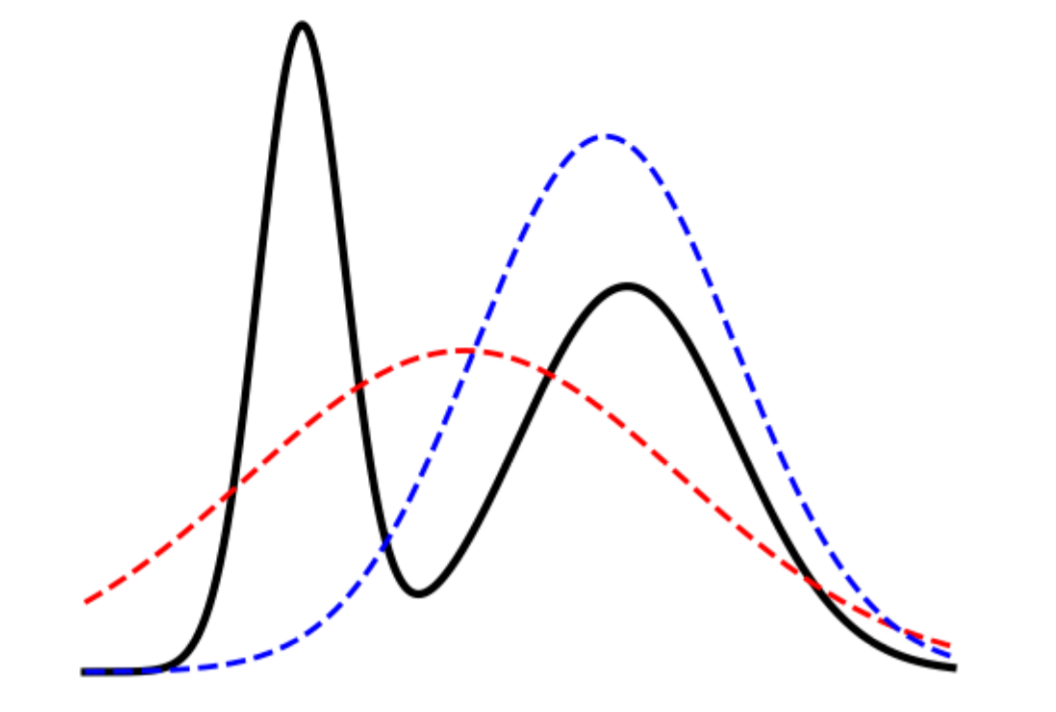
\includegraphics[scale=0.5]{images/zhang_et_al.PNG}
    \caption{Figure 1 from \cite{zhang2019variational}:  Fitting a Gaussian to a mixture of Gaussians (black) by
minimizing the forward KL (red) and the reverse KL (blue).}
    \label{fig:babrber_kl}
\end{figure}

It is a well studied fact that minimising the reverse KL that is $\argmin_{\Q \in \cdot }$ $\KL(\Q ||\P)$ can be prone to mode collapse \citep{zhang2019variational}. The issue arises from the expectations and extremisations are both taken with respect to $\Q$ and thus we can set the measure $\Q$ to 0 for regions where $\P$ has mass without incurring any penalty what so ever since this zeroes out the cost over that region. This is different to the forward KL (i.e. Maximum Likelihood)  $\argmin_{\P \in \cdot }\KL(\Q ||\P)$  which blows up  when $\P$ tries to assign $0$ to regions where $\Q$ has mass.

As put succinctly in \cite{lawrence2001variational}:

\textit{"In other words, when the approximating distribution is not
well matched to the true posterior, the former case is likely to produce a very implausible inference.
The latter case will only produce plausible inference, in legal terms it would find the truth, nothing
but the truth, but not the whole truth."}

Meaning that the reverse KL provides you with the truth (it is precise ), yet  it does not provide you with the whole truth (i.e. does not cover the whole space, has low recall).


\section{Maximum Likelihood Approach \citep{pavon2018data}}

The Approach proposed in \cite{pavon2018data} is an adaptation of Fortet's algorithm (Algorithm \ref{alg:fortet}) to the Empirical setting and is based on the following unstated observation:
\begin{observation}\label{obs:pavon}
Steps 3 and 5 of Algorithm \ref{alg:fortet}:
\begin{align}
    \hphi_0^{(i)}(\vx) := \frac{\pi_0(\vx)}{\phi_0^{(i)}(\vx)} \label{eq:term1}\\    \quad \phi_1^{(i)}(\vy) := \frac{\pi_1(\vy)}{\hphi_1^{(i)}(\vy)}  \label{eq:term2}
\end{align}
can equivalently be stated as a cross entropy minimisation problem over the space of probability distributions $\calH$:
\begin{align} \label{eq:pavon_cros_ent}
   \hphi_0^{(i)}(\vx)= \argsup_{\hphi_0(\vx) \in \calH} \E_{\pi_0(\vx)} \left[\log \hphi_0(\vx)   \phi_0^{(i)}(\vx)\right]\\
   \phi_1^{(i)}(\vy)= \argsup_{\phi_1(\vy) \in \calH} \E_{\pi_1(\vy)} \left[\log \phi_1(\vy)   \hphi_1^{(i)}(\vy)\right].
\end{align}
\end{observation}
\begin{proof}
Equation \ref{eq:term1}  implies the following:
\begin{align}\label{eq:zero}
    \KL\left(\pi_0(\vx) || \hphi_0^{(i)}(\vx)   \phi_0^{(i)}(\vx) \right)  = 0 ,
\end{align} 
% \phi_0^{(i)}(\vx) 
which can be restated as
\begin{align}
   \hphi_0^{(i)}(\vx) = \arginf_{\hphi_0(\vx)\in \mathcal{H}} \KL\left(|\pi_0(\vx) || \hphi_0(\vx)   \phi_0^{(i)}(\vx) \right),  
\end{align} 
then removing the constant entropy term we arrive at:
\begin{align*}
   \hphi_0^{(i)}(\vx)= \arginf_{\hphi_0(\vx) \in \calH} -\E_{\pi_0(\vx)} \left[\log \hphi_0(\vx)   \phi_0^{(i)}(\vx)\right]
\end{align*}
A similar argument follows for Equation \ref{eq:term2}
\end{proof}
Note that Equation \ref{eq:zero} motivates the use of other probability metrics/divergences as long as they share the same property of being minimised  when its arguments are equal. Then following Observation \ref{obs:pavon} the core escense of the method in \cite{pavon2018data} is parametrising  $\hphi_0(\vx), \;  \phi_1(\vy) $ with a parametric family of positive functions and minimise an empirical estimate of Equation \ref{eq:pavon_cros_ent}:
\begin{align}
    \hat{\beta}^*_i = \argmax_{\hat{\beta} } &\frac{1}{M} \sum_s \log \hphi_0(\vx_s; \hat{\beta} )   \phi_0^{(i)}(\vx_s)
    \quad \vx_s\sim \pi_0(\vx) \nonumber \\
   & s.t. \text{ }  \int \hphi_0(\vx; \hat{\beta} )   \phi_0^{(i)}(\vx) d\vx =1
\end{align}
and
\begin{align}
    {\beta}^*_i = \argmax_{{\beta} } &\frac{1}{N} \sum_s \log \phi_1(\vy_s; {\beta} )   \hphi_1^{(i)}(\vy_s)
    \quad \vy_s\sim \pi_1(\vy) \nonumber \\
   & s.t. \text{ }  \int \phi_1(\vy; {\beta} )   \hphi_1^{(i)}(\vy) d\vy =1
\end{align}
Furthermore via the method of Lagrange multipliers \cite{pavon1991free} show that the above two objectives can be reduced to:
\begin{align}
    \hat{\beta}^*_i = \argmax_{\hat{\beta} } &\frac{1}{M} \sum_s \log \hphi_0(\vx_s; \hat{\beta} )   \phi_0^{(i)}(\vx_s)- \int \hphi_0(\vx; \hat{\beta} )   \phi_0^{(i)}(\vx) d\vx ,
    \quad \vx_s\sim \pi_0(\vx)   \nonumber 
\end{align}
and
\begin{align}
    {\beta}^*_i = \argmax_{{\beta} } &\frac{1}{N} \sum_s \log \phi_1(\vy_s; {\beta} )   \hphi_1^{(i)}(\vy_s)- \int \phi_1(\vy; {\beta} )   \hphi_1^{(i)}(\vy) d\vy ,
    \quad \vy_s\sim \pi_1(\vy) \nonumber 
\end{align}
Now all that is left to numerically carry out this approximate variant of fortets algorithm is to estimate the propagation terms $ \phi_0^{(i)}(\vx_s), \hphi_1^{(i)}(\vy_s)$ and incorporate the constraint $\int \phi_1(\vy; {\beta} )   \hphi_1^{(i)}(\vy) d\vy, \, \int \hphi_0(\vx; \hat{\beta} )   \phi_0^{(i)}(\vx) d\vx $ which depend on a non-trivial multidimensional integral.


\subsection{Importance Sampling Approach by \citet{pavon2018data} }

Estimating the terms $ \phi_0^{(i)}(\vx_s), \hphi_1^{(i)}(\vy_s)$, can be done without much trouble as they are effectively expectations with respect to the prior which we can sample from either directly in the case of Brownian motion or via the EM discretisation for more complex Ito-process prios. Furthermore in \cite{pavon1991free} they only estimate the term $\hphi_1^{(i)}(\vy_s)$:

\begin{align}\label{eq:pavon_transition_mc}
    \phi_1^{(i)}(\vx_s) &= \int P(\vy| \vx_s) \phi_1^{(i)}(\vy; \beta) d\vy \nonumber \\
    &\approx \frac{1}{\tilde{M}} \sum_l \phi_1^{(i)}(\tilde{\vy}_{ls}; \beta) \quad \tilde{\vy}_{ls} \sim   P(\vy| \vx_s)
\end{align}

as we require only one of the propagations in order to compute the normalising constraints  $\int \phi_1(\vy; {\beta} )   \hphi_1^{(i)}(\vy) d\vy , \, \int \hphi_0(\vx; \hat{\beta} )   \phi_0^{(i)}(\vx) d\vx $.

\cite{pavon2018data} Note that the integrals arising from the constraint can be decomposed in the following convenient order:
\begin{align}
\int \hphi_0(\vx; \hat{\beta} )   \phi_0^{(i)}(\vx) d\vx &=\nonumber\\
& = \int  \hphi_0(\vx; \hat{\beta} ) \int P(\vy| \vx_s) \phi_1^{(i)}(\vx; \beta) d\vy d\vx \\
    \int \phi_1(\vy; {\beta} )   \hphi_1^{(i)}(\vy) d\vy &=\nonumber\\
    &=\int  \hphi_0(\vx; \hat{\beta} ) \int P(\vy| \vx_s) \phi_1^{(i)}(\vx; \beta) d\vy d\vx.
\end{align}
Now all that is required is estimating the outer integrals with respect to $d\vx$ as we have already provided a Monte-Carlo estimate for the $d\vy$ integral in Equation \ref{eq:pavon_transition_mc}. In order to estimate the outer integrals  \cite{pavon2018data} propose to use a method of importance sampling:
\begin{align}
    \int&  \hphi_0(\vx; \hat{\beta} ) \int P(\vy| \vx_s) \phi_1^{(i)}(\vx; \beta) d\vy d\vx = \nonumber \\
    & = \int \tilde{\pi}_0(\vx) \frac{\hphi_0(\vx; \hat{\beta} ) \int P(\vy| \vx_s) \phi_1^{(i)}(\vx; \beta) d\vy}{\tilde{\pi}_0(\vx)} d\vx \nonumber \\ 
     &\approx  \frac{1}{\tilde{M}\tilde{N}}\sum_{lk} \frac{\hphi_0(\vx_k; \hat{\beta} )\phi_1^{(i)}(\tilde{\vy}_{lk}; \beta) }{\tilde{\pi}_0(\vx_k)} ,  \quad \vy_{lk} \sim   P(\vy| \vx_k), \, \vx_k\sim\tilde{\pi}_0(\vx),
\end{align}
where the authors of \cite{pavon2018data} recommend  to set  $\tilde{\pi}_0(\vx)$ to a density estimator of $\pi_0(\vx)$ since the integrand  $\hphi_0(\vx; \hat{\beta} )\phi_0^{(i)}(\vx)$ will converge  to a density estimator for  $\pi_0(\vx)$ as we iterate Fortet's algorithm. However in the early iterations of Fortet's algorithm there is no particular advantage in this heuristic to initialise the importance sampler. Furthermore this naive importance sampling scheme does not take into account sampling in areas where the integrand has mass (i.e. near its modes for example). Another comment is that due to the curse of dimensionality vanilla importance samplers will not scale to high dimensions.


\subsection{Alternative Formulation as an Unnormalised Likelihood Problem}

Rather than enforcing the integrate to one constraint via a method of Lagrange multipliers we can enforce it via the following reparametrisation:
\begin{align}
    \hat{\beta}^*_i = \argmax_{\hat{\beta} } &\frac{1}{M} \sum_s \log \frac{\hphi_0(\vx_s; \hat{\beta} )   \phi_0^{(i)}(\vx_s)}{ \int \hphi_0(\vx; \hat{\beta} )   \phi_0^{(i)}(\vx) d\vx}
    \quad \vx_s\sim \pi_0(\vx) \nonumber 
\end{align}
and
\begin{align}
    {\beta}^*_i = \argmax_{{\beta} } &\frac{1}{N} \sum_s \log\frac{ \phi_1(\vy_s; {\beta} )   \hphi_1^{(i)}(\vy_s)}{ \int \phi_1(\vy; {\beta} )   \hphi_1^{(i)}(\vy) d\vy }
    \quad \vy_s\sim \pi_1(\vy) \nonumber 
\end{align}

Turning the problem into estimating and fitting an un-normalised likelihood \cite{gutmann2010noise}. This formulation opens up the door to alternate estimation techniques to maximum likelihood such as Noise Contrastive Estimation \cite{gutmann2010noise}.

\subsection{Analysis of simple Gaussian like Parametrisation}

Following the reparamtrisation introduced in the previous section we consider the case of parametrising the potentials with unimodal Gaussian's this allows for further analysis of the method since both the normalisation and the updates can be attained in closed form. 

Firstly we put forward the following counter example that valid Gaussian like parametrisation's for the potentials cannot solve the bridge even for uni-modal Gaussian marginals:
\begin{proposition}
If we parametrise the potentials as:
\begin{align}
\hphi_0( \vx ; \beta) =  \calN(\vx | \vmu_x, \mSigma_x) \\
\phi_1( \vy ; \hat{\beta}) =  \calN(\vy | \vmu_y, \mSigma_y) 
\end{align}
and try to solve the Empirical bridge for the marginals:
\begin{align*}
    \pi_0(x) =  \mathcal{Z}_x^{-1}\calN(x,0, 1) \\
    \pi_1(y) = \mathcal{Z}_y^{-1} \calN(y,0, 10^2) 
\end{align*}
then the MLE based approximation of Fortet's in \cite{pavon2018data} will not meet the marginal constraints.
\end{proposition}
\begin{proof}
 Assuming a Brownian motion $\W^{\gamma}$ Propagating:
\begin{align*}
\phi_0( \vx ; \hat{\beta}) = \mathcal{Z}_x^{-1} \calN(\vx| \vmu_y, \mSigma_y + \gamma \I)  \\
{\hphi}_1( \vy ; {\beta}) = \mathcal{Z}_y^{-1}  \calN(\vy| \vmu_x, \mSigma_x + \gamma \I) 
\end{align*}
Then:
\begin{align*}
 \phi_0( \vx ; \hat{\beta})  \phi_0(\vx ; \beta) = \calN\Big(\vx \Big|& \big(\mSigma_x^{-1} + (\mSigma_y + \gamma \I)^{-1}\big)^{-1}\big( \mSigma_x^{-1}\vmu_x + (\mSigma_y + \gamma \I)^{-1}\vmu_y)\big), \\ &\big(\mSigma_x^{-1} + (\mSigma_y + \gamma \I)^{-1}\big)^{-1} \Big)
\end{align*}
Via MLE (holding $y$-params constant)we have:
\begin{align*}
\left(\mSigma_x^{-1} + (\mSigma_y + \gamma \I)^{-1}\right)^{-1}  = \mS_x 
\end{align*}
Yielding update
\begin{align*}
\mSigma_x^{(t)} = (\mS_x^{-1}  - (\mSigma_y^{(t-1)} + \gamma \I)^{-1})^{-1} 
\end{align*}
and 
\begin{align*}
\left(\mSigma_x + (\mSigma_y + \gamma \I)^{-1}\right)^{-1}\left( \mSigma_x^{-1}\vmu_x + (\mSigma_y + \gamma \I)^{-1}\vmu_y)\right) = \bar{\vx} \\
\left( \mSigma_x^{-1}\vmu_x + (\mSigma_y + \gamma \I)^{-1}\vmu_y)\right) = \left(\mSigma_x^{-1} + (\mSigma_y + \gamma \I)^{-1}\right)\bar{\vx} 
\end{align*}
Yielding update:
\begin{align*}
\vmu_x^{(i)}  = \left(\mathbb{I} + \mSigma_x^{(i)}(\mSigma_y^{(i-1)} + \gamma \I)^{-1}\right)\bar{\vx} -  \mSigma_x^{(i)}(\mSigma_y^{(i-1)} + \gamma \I)^{-1}\vmu_y^{(i-1)}
\end{align*}
and similarity  for $\mSigma_y, \vmu_y$.
In 1D (and in terms of the free paramters) the fitted marginal desnity variances are:
\begin{align*}
\sigma_y^{*} = \left(\frac{1}{1+\sigma^2_x} + \frac{1}{\sigma^2_y}\right)^{-1} \\
\sigma_x^{*} = \left(\frac{1}{1+\sigma^2_y} + \frac{1}{\sigma^2_x}\right)^{-1}
\end{align*}
If the empirical marginal variances were $1,10$ :
\begin{align*}
1 = \left(\frac{1}{1+\sigma^2_x} + \frac{1}{\sigma^2_y}\right)^{-1} \\
10 = \left(\frac{1}{1+\sigma^2_y} + \frac{1}{\sigma^2_x}\right)^{-1}
\end{align*}
Then the above system has no valid solutions (can be solved only for negative values of $\sigma_x$), by the quadratic formula:
\begin{align*}
0.8 \sigma_x^4 + 1.9 \sigma_x^2 + 1 = 0 \quad \quad \quad \text{\Lightning}
\end{align*}

\end{proof}

In short what the above tells us is that if we wish to do a squared exponential paremetrisation for the potentials we must drop the positive definite constraint . In geometric terms if one potential is log concave then the other needs to be log convex due to how the variances combine.

We still however must enforce an integrability constraint (required to make the inner product of potentials converge):
\begin{align*}
\left(\mSigma_x^{-1} +\mSigma_y^{-1}\right)^{-1} = \mL\mL^{\top}
\end{align*}
which implies:
\begin{align*}
\mSigma_x^{-1} +\mSigma_y^{-1} = \mL\mL^{\top}
\end{align*}
which can be enforced via a simple reparametrisation (this allows for negative lengthscales):
\begin{align*}
\mSigma_x = (\mL\mL^{\top} -\mSigma_y^{-1})^{-1}
\end{align*}
Where $\mL$ can be paramterised in terms of an unconstrained vector.
\subsection{Mixture of Exponentiated Quadratics}


We now wish to consider if its possible to extend the exponentiated quadratic  parametrisation of the potentials to a mixture of exponentiated quadratics. In order to achieve this parametrisation we need to reconsider the integrability constraint.
\subsection{Noise Contrastive Estimation}
\section{Comparison of Approaches}

%\chapter{Evaluation} 
\chapter{Experiments}

%\chapter{Summary and Conclusions} 
\chapter{Discussion}


\appendix
\singlespacing

\bibliographystyle{icml} 
\bibliography{bibliography} 

\end{document}
